%%%%%%%%%%%%%%%%%%%%%%%%%%%%%%%%%%%%%%%%%%%%%%%%%%%%%%%%%%%%%%%%%%%%%%%%%%%%%%%%%%%%%%%%%%%%%%%%%%%%%%%%%%%%%%%%%%%%%%%%%%%%%%%%%%%%%%%%%%%%%%%%%%%%%%%%%%%
% This is just an example/guide for you to refer to when submitting manuscripts to Frontiers, it is not mandatory to use Frontiers .cls files nor frontiers.tex  %
% This will only generate the Manuscript, the final article will be typeset by Frontiers after acceptance.
%                                              %
%                                                                                                                                                         %
% When submitting your files, remember to upload this *tex file, the pdf generated with it, the *bib file (if bibliography is not within the *tex) and all the figures.
%%%%%%%%%%%%%%%%%%%%%%%%%%%%%%%%%%%%%%%%%%%%%%%%%%%%%%%%%%%%%%%%%%%%%%%%%%%%%%%%%%%%%%%%%%%%%%%%%%%%%%%%%%%%%%%%%%%%%%%%%%%%%%%%%%%%%%%%%%%%%%%%%%%%%%%%%%%

%%% Version 3.4 Generated 2018/06/15 %%%
%%% You will need to have the following packages installed: datetime, fmtcount, etoolbox, fcprefix, which are normally inlcuded in WinEdt. %%%
%%% In http://www.ctan.org/ you can find the packages and how to install them, if necessary. %%%

\documentclass[utf8]{frontiersSCNS}

%\setcitestyle{square} % for Physics and Applied Mathematics and Statistics articles
\usepackage{url,hyperref,lineno,microtype,subcaption}
\usepackage[onehalfspacing]{setspace}

\linenumbers


% BELOW TAKEN FROM rticles plos template
%
% amsmath package, useful for mathematical formulas
\usepackage{amsmath}
% amssymb package, useful for mathematical symbols
\usepackage{amssymb}

% hyperref package, useful for hyperlinks
\usepackage{hyperref}

% graphicx package, useful for including eps and pdf graphics
% include graphics with the command \includegraphics
\usepackage{graphicx}

% Sweave(-like)
\usepackage{fancyvrb}
\DefineVerbatimEnvironment{Sinput}{Verbatim}{fontshape=sl}
\DefineVerbatimEnvironment{Soutput}{Verbatim}{}
\DefineVerbatimEnvironment{Scode}{Verbatim}{fontshape=sl}
\newenvironment{Schunk}{}{}
\DefineVerbatimEnvironment{Code}{Verbatim}{}
\DefineVerbatimEnvironment{CodeInput}{Verbatim}{fontshape=sl}
\DefineVerbatimEnvironment{CodeOutput}{Verbatim}{}
\newenvironment{CodeChunk}{}{}

% cite package, to clean up citations in the main text. Do not remove.
\usepackage{cite}

\usepackage{color}

\providecommand{\tightlist}{%
  \setlength{\itemsep}{0pt}\setlength{\parskip}{0pt}}

% Below is from frontiers
%
\bibliographystyle{frontiersinSCNS}
% Use doublespacing - comment out for single spacing
%\usepackage{setspace}
%\doublespacing


% Leave a blank line between paragraphs instead of using \\


\def\keyFont{\fontsize{8}{11}\helveticabold }


%% ** EDIT HERE **
%% PLEASE INCLUDE ALL MACROS BELOW

%% END MACROS SECTION

% Pandoc citation processing
\newlength{\csllabelwidth}
\setlength{\csllabelwidth}{3em}
\newlength{\cslhangindent}
\setlength{\cslhangindent}{1.5em}
% for Pandoc 2.8 to 2.10.1
\newenvironment{cslreferences}%
  {}%
  {\par}
% For Pandoc 2.11+
\newenvironment{CSLReferences}[2] % #1 hanging-ident, #2 entry spacing
 {% don't indent paragraphs
  \setlength{\parindent}{0pt}
  % turn on hanging indent if param 1 is 1
  \ifodd #1 \everypar{\setlength{\hangindent}{\cslhangindent}}\ignorespaces\fi
  % set entry spacing
  \ifnum #2 > 0
  \setlength{\parskip}{#2\baselineskip}
  \fi
 }%
 {}
\usepackage{calc} % for calculating minipage widths
\newcommand{\CSLBlock}[1]{#1\hfill\break}
\newcommand{\CSLLeftMargin}[1]{\parbox[t]{\csllabelwidth}{#1}}
\newcommand{\CSLRightInline}[1]{\parbox[t]{\linewidth - \csllabelwidth}{#1}\break}
\newcommand{\CSLIndent}[1]{\hspace{\cslhangindent}#1}
\usepackage{booktabs}
\usepackage{longtable}
\usepackage{array}
\usepackage{multirow}
\usepackage{wrapfig}
\usepackage{float}
\usepackage{colortbl}
\usepackage{pdflscape}
\usepackage{tabu}
\usepackage{threeparttable}
\usepackage{threeparttablex}
\usepackage[normalem]{ulem}
\usepackage{makecell}
\usepackage{xcolor}


\def\Authors{
  Maxwel C Oliveira\,\textsuperscript{1},
  Amit J Jhala\,\textsuperscript{2},
  Mark Bernards\,\textsuperscript{3},
  Chris Proctor\,\textsuperscript{2},
  Strahinja Stepanovic\,\textsuperscript{2},
  Rodrigo Werle\,\textsuperscript{1*}}

\def\Address{

  \textsuperscript{1} Department of Agronomy, University of
Wisconsin-Madison,  Madison,  Wisconsin,  United States
  
  \textsuperscript{2} Department of Agronomy and
Horticulture, University of
Nebraska-Lincoln,  Lincoln,  Nebraska,  United States
  
  \textsuperscript{3} Department of Agronomy, Western Illinois
University,  Macomb,  Illinois,  United States
  }

  
  \def\firstAuthorLast{Oliveira {et~al.}}
  
  
  
  
  
  
  
  
  \def\corrAuthor{Rodrigo Werle}\def\corrAddress{Department of Agronomy,
University of Wisconsin-Madison, United States\\1575 Linden
Dr\\Madison, Wisconsin, 53705 United
States}\def\corrEmail{\href{mailto:rwerle@uwisc.edu}{\nolinkurl{rwerle@uwisc.edu}}}
  


\begin{document}
\onecolumn
\firstpage{1}

\title[Palmer amaranth adaptation]{Palmer amaranth (\emph{Amaranthus
palmeri}) adaptation to US Midwest agroecosystems}
\author[\firstAuthorLast]{\Authors}
\address{} %This field will be automatically populated
\correspondance{} %This field will be automatically populated

\extraAuth{}% If there are more than 1 corresponding author, comment this line and uncomment the next one.
%\extraAuth{corresponding Author2 \\ Laboratory X2, Institute X2, Department X2, Organization X2, Street X2, City X2 , State XX2 (only USA, Canada and Australia), Zip Code2, X2 Country X2, email2@uni2.edu}


\maketitle

\begin{abstract}

Palmer amaranth (\emph{Amaranthus palmeri} S. Watson) is one of the most troublesome weed species in the United States. Palmer amaranth is endemic to Southern United States but its range is expanding northward. Palmer amaranth dispersal warrants studies assessing species adaptation into new geographies. A study was conducted to investigate morphology, flowering and sex dimorphism from cohorts of Palmer amaranth growing under corn, soybean, and bareground across five locations of US Midwest. Results demonstrated that first cohort of Palmer amaranth, established in June, produced 42\% more biomass than plants from second cohort (established in July). The first Palmer amaranth cohort produced 75.5 g plant\textsuperscript{-1} in bareground, 28.3 g plant\textsuperscript{-1} in soybean and 16.3 g plant\textsuperscript{-1} in corn, whereas the second Palmer amaranth cohort produced 62.6, 6.3, and 1.4 g plant\textsuperscript{-1} in bareground, soybean and corn, respectively. Palmer amaranth height was more impacted when growing in corn. Palmer amaranth plants averaged 85.2 cm tall in the first cohort but 38.2 cm tall in the second cohort in corn. Moreover, Palmer amaranth flowering window shifted according to crop and cohort timings. Palmer amaranth growing in intense competition, such as under low light in corn, resulted in the longest flowering window. Also, Palmer amaranth sex dimorphism was slightly influenced by day of year, weight and height. The model estimated that probability of being a female plant increased as biomass and height increased. Our results showed the fast adaptation and plasticity of Palmer amaranth to grow and adapt to cropping systems from the US Midwest. Palmer amaranth is likely to continue its expansion northward. Therefore, preventing plant dispersal into new habitats is the most effective management strategy. Reactive management to reduce Palmer amaranth impact on cropping systems should encompass diversity of tactics that minimize the species ability to establish into cropping systems, including crop rotation (beyond corn and soybean), early/late crop planting, row spacing, cover crops, and effective chemical control programs.

\tiny
 \keyFont{ \section{Keywords:} Evolution, Flowering, Management, Pigweed, Weed} 

\end{abstract}

\hypertarget{introduction}{%
\section*{Introduction}\label{introduction}}
\addcontentsline{toc}{section}{Introduction}

Palmer amaranth (\emph{Amaranthus palmeri} S. Watson) is currently
ranked as one of the most economically detrimental weed species to
cropping systems in the United States (Van Wychen, 2020). Unmanaged
Palmer amaranth plants compete for water, light, and nutrients, which
can drastically impact crop yields (Berger et al., 2015). For example,
Palmer amaranth has been documented to reduce up to 91\%, 68\%, and 54\%
corn (Massinga et al., 2001), soybean (Klingaman and Oliver, 1994), and
cotton (Morgan et al., 2001) yields, respectively. Moreover, Palmer
amaranth has shown a remarkable capacity to evolve resistance to
herbicides. To date, Palmer amaranth has evolved resistance to eight
herbicide sites of action (Heap, 2021), increasing the weed management
complexity (Lindsay et al., 2017). Thus, Palmer amaranth poses an
economical and environmental risk to sustainable agriculture.

Palmer amaranth is a fast growing summer annual forb indigenous to the
Sonoran Desert (Sauer, 1957). The species would eventually emerge as a
threat to US agriculture in the 1990s. Palmer amaranth weediness is
likely a result of human-assisted selection in combination with plant
biology. Farm mechanization, adoption of conservation agriculture (e.g.,
no-till), and intensive use of herbicides for weed management are the
main human-mediated selection of Palmer amaranth into cropping systems
(Ward et al., 2013). On the other hand, Palmer amaranth is a prolific
seed producer with a C4 photosynthetic apparatus (Wang et al., 1992).
With a dioecy nature, Palmer amaranth male and female plants are
obligate outcrosser species, increasing the chances of exchanging
adaptive traits among plants (Jhala et al., 2021; Oliveira et al.,
2018). Also, Palmer amaranth small seeds (e.g, 1 mm) tend to thrive in
no-tillage systems (Price et al., 2011), and spread across locations
through farm equipment (Sauer, 1972), manure (Hartzler and Anderson,
2016), wildlife (Farmer et al., 2017), etc. The dispersal capacity of
Palmer amaranth makes the species one of the most successful cases of
weed adaptation to current cropping systems.

Light and temperature are the main environmental requirements for Palmer
amaranth growth and development (Jha et al., 2010). Palmer amaranth is
reported with an extended germination period (Ward et al., 2013).
Germination of Palmer amaranth was triggered by 18 C soil temperature at
5 cm depth (Keeley et al., 1987), and optimal germination and biomass
production occurred at 35/30 C day and night temperatures (Guo and
Al-Khatib, 2003). In addition, Palmer amaranth establishment is
human-mediated by tillage timings and preemergence-applied herbicides
(Chahal et al., 2021), which can result in weed germination shifts
(Sbatella and Wilson, 2010). Soil water content has not shown to limit
Palmer amaranth fitness. Under continuous water stress, Palmer amaranth
survived and produced at least 14000 seeds plant\textsuperscript{-1}
(Chahal et al., 2018). Seeds from Palmer amaranth growing with limited
water conditions were heavier, less dormant, and prompt for germination
(Matzrafi et al., 2021). Growing conditions and management practices
also influence Palmer amaranth sex dimorphism and flowering pattern
(Korres et al., 2017; Rumpa et al., 2019). Therefore, Palmer amaranth
has shown plasticity to evolve and fast adapt under the current
agroecosystem conditions. Further scenarios show that global temperature
warming can impact agriculture, and promote niches for Palmer amaranth
invasion/adaptation into new environments. Currently, it is estimated
that the greatest climatic risk of Palmer amaranth establishment are
agronomic crops in Australia and Sub-Sahara Africa (Kistner and
Hatfield, 2018). Temperature is a key factor limiting Palmer amaranth
expansion to cooler geographies (Briscoe Runquist et al., 2019);
however, under future climate change Palmer amaranth is likely to expand
northward into Canada and Northern Europe (Kistner and Hatfield, 2018;
Briscoe Runquist et al., 2019).

Palmer amaranth is already found in agronomic crops of South America
(Larran et al., 2017; Küpper et al., 2017) and Southern Europe (Milani
et al., 2021). In the United States, Palmer amaranth is well established
in the Cotton Belt (Garetson et al., 2019; Bagavathiannan and
Norsworthy, 2016) in the southern United States but its range is
expanding northward. For example, herbicide resistant Palmer amaranth is
widespread in Nebraska (Oliveira et al., 2021). There are some reported
cases of Palmer amaranth in Michigan (Kohrt et al., 2017) and
Connecticut (Aulakh et al., 2021). Also, it is estimated that Palmer
amaranth can cause high damage to soybean fields in Illinois (Davis et
al., 2015), which is concerning as soybean along with corn make most of
US Midwest agronomic hectares. In Iowa, a study showed that Palmer
amaranth is still not well adapted compared to waterhemp
(\emph{Amaranthus tuberculatus}) (Baker, 2021). Waterhemp, an
\emph{Amaranthus} species, is the most troublesome species in the US
Midwest (Tranel et al., 2011). Nonetheless, invasion and successful
eradication of Palmer amaranth is documented in Minnesota (Yu et al.,
2021). Palmer amaranth infestations have not been detected in Canada;
however, Palmer amaranth seeds were detected in sweet potato slips in
the country (Page et al., 2021). Palmer amaranth is still not as well
adapted and established to Northern as it is in the Southern North
America. Therefore, Palmer amaranth range of expansion into new habitats
can increase. It seems certain the need to manage new Palmer amaranth
infestations in agronomic crops throughout northern United States in the
near future. Strategies on Palmer amaranth management should encompass
the agroecosystem level but not only attempts to eradicate the weed.
Most tactics to manage Palmer amaranth are based on technology fixes
(Scott, 2011), which are short-term (e.g., herbicide and/or tillage)
rather than long-term weed management. Palmer amaranth management should
be built on minimizing the species ability to adapt, grow and develop
into agroecossystems.

In the southeastern US, early growing Palmer amaranth is well known to
have a higher impact on cotton yields compared to late established
plants (MacRae et al., 2013). In the northern states, Palmer amaranth
impact on the agroecosystem is recent. Studies investigating Palmer
amaranth in those locations are limited due to the plant classification
as noxious weed species in some northern states (Yu et al., 2021).
Nonetheless, the continuous Palmer amaranth dispersal and potential
establishment across the northern United States is concerning and
warrants investigations on species morphology in such environments.
Understanding Palmer amaranth biology and growing strategies under
different agroecosystems can enhance our knowledge on species adaptation
and management practices. It can also aid in designing proactive and
ecological tactics to limit the species range expansion, reduce its
negative impact, and developing resilient and sustainable farming
systems (MacLaren et al., 2020). Therefore, the objective of this study
was to investigate the flowering pattern, sex dimorphism, biomass
production, and height of Palmer amaranth cohorts growing under corn,
soybean and bareground across five locations in the United States
Midwest.

\hypertarget{material-and-methods}{%
\section*{Material and Methods}\label{material-and-methods}}
\addcontentsline{toc}{section}{Material and Methods}

\hypertarget{plant-material-and-growing-conditions}{%
\subsection*{Plant material and growing
conditions}\label{plant-material-and-growing-conditions}}
\addcontentsline{toc}{subsection}{Plant material and growing conditions}

A Palmer amaranth accession (Kei3) from Perkins County, Nebraska with no
glyphosate resistance according to Oliveira et al. (2021) was selected
for this study. Three weeks prior to the establishment of each cohort,
seeds were planted in plastic trays containing potting-mix. Emerged
seedlings (1 cm) were transplanted into 200 cm\textsuperscript{-3}
plastic pots (a plant pot\textsuperscript{-1}). Palmer amaranth
seedlings were supplied with adequate water and kept under greenhouse
conditions at the University of Wisconsin-Madison, University of
Nebraska-Lincoln, and Western Illinois University; and kept outdoors at
the Perkins extension office in Grant, NE until the 2-3 leaf stage (5 to
8 cm height) when they were transported to the field.

\hypertarget{field-study}{%
\subsection*{Field study}\label{field-study}}
\addcontentsline{toc}{subsection}{Field study}

The experiment was conducted in 2018 and 2019 under field conditions at
five locations: Arlington, WI (43°18'N, 89°29'W), Clay Center, NE
(40.57'N, 9814'W), Grant, NE (XXX'N, XXX'W), Lincoln, NE (41.16'N,
96.42'W), and Macomb, IL (XXX'N, XXX'W).

Fields were conventionally tilled prior to crop planting. Corn and
soybean were planted in 76-cm row spacing (Table 1). Monthly mean air
temperature and total precipitation were obtained using Daymet weather
data from June through September across the five locations in 2018 and
2019 (Correndo et al., 2021) (Figure 1)

\begin{table}[!h]

\caption{\label{tab:unnamed-chunk-2}Field study attributes from Arlington, WI, Clay Center, NE, Grant, NE, Lincoln, NE and Macomb, IL}
\centering
\resizebox{\linewidth}{!}{
\fontsize{10}{12}\selectfont
\begin{tabular}[t]{lllllll}
\toprule
Attributes &  & Arlington, WI & Clay Center, NE & Grant, NE & Lincoln, NE & Macomb, IL\\
\midrule
Bareground &  &  &  &  &  & \\

 & Weed control & glyphosate\textsuperscript{a} / \emph{S}-metolachor\textsuperscript{b} & saflufenacil + imazethapyr + pyroxasulfone\textsuperscript{c} &  &  & \\

Corn &  &  &  &  &  & \\

 & Hybrid & NK0142 3120-EZ1 & DKC60-67 &  &  & \\

 & Seeding rate & 88956 & 86487 &  &  & \\

 & Weed control & glyphosate / \emph{S}-metolachor & \emph{S}-metolachlor + trazine + mesotrione + bicyclopyrone\textsuperscript{d} &  &  & \\

 & Stage at 1\textsuperscript{st} cohort & V2-3 &  &  &  & \\

 & Stage at 2\textsuperscript{nd} cohort & V6-7 &  &  &  & \\

 & Planting day & April 30, 2018 / May 5, 2019 & May 10, 2018/19 &  &  & \\

\multirow{-7}{*}{\raggedright\arraybackslash } & Fertilization & N (46-0-0) at 157 kg ha\textsuperscript{-1} &  &  &  & \\

Soybean &  &  &  &  &  & \\

 & Variety & DSR-1950 & AG21X8 &  &  & \\

 & Seeding rate & 296400 & 321237 &  &  & \\

 & Weed control & glyphosate / \emph{S}-metolachor & saflufenacil + imazethapyr + pyroxasulfone &  &  & \\

 & Stage at 1\textsuperscript{st} cohort & V1-2 &  &  &  & \\

 & Stage at 2\textsuperscript{nd} cohort & V5-6 &  &  &  & \\

\multirow{-6}{*}{\raggedright\arraybackslash } & Planting day & May 5, 2018 / May 10, 2009 & May 14, 2018/19 &  &  & \\

Soil &  &  &  &  &  & \\

 & Type & Plano-silt-loam & Crete Silt Loam &  &  & \\

 & Ratio (sand-clay-silt) & 10-64-26 & 17-58-25 &  &  & \\

 & pH & 6.6 & 6.5 &  &  & \\

\multirow{-4}{*}{\raggedright\arraybackslash } & Organic matter (\%) & 3.5 & 3 &  &  & \\
\bottomrule
\multicolumn{7}{l}{\rule{0pt}{1em}\textsuperscript{a} glyphoste, 840 g ae ha \textsuperscript{b} \emph{S}--metolachor, 1324 g ai ha; \textsuperscript{c} saflufenacil + imazethapyr + pyroxasulfone, 215 g ai ha; \textsuperscript{d} \emph{S}-metolachlor + trazine + mesotrione, + bicyclopyrone, 2409 g ai ha}\\
\end{tabular}}
\end{table}

The field experimental units were three adjacent 9.1 m wide (12 rows at
76.2 cm row spacing) by 10.7 m long. The experimental design were
arranged in factorial design with three crops, two transplanting times
simulating two cohorts, repeated across five locations. Each filed
experimental unit was planted with corn, soybean, or kept under
bareground. The two transplant timings were June 1 (first cohort) and
July 1 (second cohort). Palmer amaranth seedlings (potting mix + two
seedlings) were transplanted (6 cm deep and 8 cm wide). Forty-eight
plants were equidistantly placed (0.76 m apart) between rows within each
crop. After a week, one plant was eliminated and one was kept, resulting
in 24 plants per experimental unit and transplanting time (Figure 2).
When needed, Palmer amaranth plants were supplied with water during the
first week after transplanting to assure seedling survival.

After transplanting, Palmer amaranth flowering was monitored until the
end of the study. When a plant flowered, the day was recorded, plant sex
was identified (male or female), plant height was measured from soil
surface to the top of plant. Also, aboveground plant biomass was
harvested near soil surface and oven dried at 65 C until reaching
constant weight before weigh (g plant\textsuperscript{-1}) was recorded.

Plants had to be harvested at flowering because Palmer amaranth is
neither endemic in Wisconsin nor in Illinois. In our study, all
locations followed the methodology of plant harvest at flowering
initiation, except in Grant, NE. In this location, all Palmer amaranth
plants were harvest at once on July 06, 2018 and 2019 (first cohort),
and on August 17, 2018 and on July 31, 2019 (second cohort).

\hypertarget{statistical-analyses}{%
\subsection*{Statistical analyses}\label{statistical-analyses}}
\addcontentsline{toc}{subsection}{Statistical analyses}

The statistical analyses were performed using R statistical software
version 4.0.1 (Team, 2021). Data analyses are stored at Zenodo
(Oliveira, 2021).

Analyses of Palmer amaranth height and biomass were performed with a
linear mixed model using \emph{lmer} function from ``lme4'' package
(Bates et al., 2015). Plant height and biomass were log transformed to
meet model assumption of normality. In the model, crop (bareground,
corn, soybean) and cohort time (first and second) were the fixed effects
and year nested with location the random effects. Analysis of variance
at \(\alpha\) 0.05 was performed with \emph{anova} function from ``car''
package (Fox and Weisberg, 2018). Marginal means and compact letter
display were estimated with \emph{emmeans} and \emph{cld} from packages
``emmeans'' (Lenth et al., 2021) and ``multcomp'' (Hothorn et al.,
2008), respectively.

The Palmer amaranth flowering timing was estimated as cumulative
flowering across all locations, except Grant, NE. Palmer amaranth
cumulative flowering estimation was determined using an asymmetrical
three parameter log logistic Weibull model of the drc package (Ritz et
al., 2015).

\[Y(x) = 0 + (d-0) exp (-exp(b(log(x)-e)))\]

In this model, \emph{Y} is the Palmer amaranth cumulative flowering,
\emph{d} is the upper limit (set to 100), and \emph{e} is the inflection
point, and \emph{x} day of year (doy).

The doy for 10, 50, and 90\% Palmer amaranth cumulative flowering were
determined using the \emph{ED} function of drc package. Also, the 10,
50, and 90\% Palmer amaranth cumulative flowering were compared among
crops and cohorts using the \emph{EDcomp} function of drc package. The
EDcomp function compares the ratio of cumulative flowering using
t-statistics, where P-value \textless{} 0.05 indicates that we fail to
reject the null hypothesis.

A binary logistic regression was fitted to Palmer amaranth sex
dimorphism. Binary logistic regression is used for predicting binary
classes (Bangdiwala, 2018), such as the probability of a plant being
female in a dioecious species. Prior to the analysis, missing values
were removed from the dataset. Also, data from Grant was not used in
this analysis due to the uniform plant harvesting at that location. The
complete dataset was splitted into 80\% train and 20\% test data. The
80\% train is used for the model training and the 20\% test is used for
checking model performance on unseen dataset. With 80\% dataset, a
generalized linear model (base R \emph{glm} function) was fitted to
binary response variable, the probability of being female (0 to male and
1 to female). The independent variables were day of year harvest,
height, weight, and crop (without interaction). The model family was
binomial with a logit function. The model fit was assessed through
pseudo R-squared values (McFadden, Cox and Snell, Cragg and Uhler) and
likelihood ratio using \emph{nagelkerke} function from ``rcompanion''
package (Mangiafico, 2021). The marginal effects computation was
performed with Average Marginal Effects (AMEs) at every observed value
of x and average across the results (Leeper, 2017) using \emph{margins}
function from ``margins'' package (Leeper et al., 2021). The 20\% test
data was predicted using the \emph{predict} function with a cutoff
estimation for male or female using \emph{performance} function from
ROCR package (Sing et al., 2005). The model quality prediction from the
classification algorithm was measured with precision (\emph{precision}
function), recall (\emph{recall} function) and F1-score (\emph{f\_meas}
function) using the ``yardstick'' package (Kuhn et al., 2021). The
precision determines the accuracy of positive predictions (female
plants), recall determines the fraction of positives that were correctly
identified, and F1-score is a weighted harmonic mean of precision and
recall with the best score of 1 and the worst score of 0 (Raoniar,
2021). F1-score conveys the balance between the precision and the recall
(Yacouby and Axman, 2020). The area under the receiver operating curve
(AUC-ROC) was also estimated with performance function using the true
positive and false positive rates. Higher the AUC, better the model is
at distinguishing between female and male Palmer amaranth.

\hypertarget{results}{%
\section*{Results}\label{results}}
\addcontentsline{toc}{section}{Results}

\hypertarget{palmer-amaranth-height-and-biomass}{%
\subsection*{Palmer amaranth height and
biomass}\label{palmer-amaranth-height-and-biomass}}
\addcontentsline{toc}{subsection}{Palmer amaranth height and biomass}

Palmer amaranth plants accumulated more biomass when growing in
bareground compared to plants growing in soybean and corn (figure 3A).
Palmer amaranth plants in the first cohort produced 75.5, 28.3, and 16.3
g plant\textsuperscript{-1} in bareground, soybean and corn,
respectively. Plants from the second cohort produced 62.6 g
plant\textsuperscript{-1} in bareground, followed by 6.3 g
plant\textsuperscript{-1} in soybean, and 1.4 g
plant\textsuperscript{-1}.

Palmer amaranth height was more uniform across cohort timings, except
when growing in corn (figure 3B). Palmer amaranth plants from the first
cohort were on average 69.2 cm tall in bareground, which was not
different from the 70.7 cm tall plants from the second cohort timing (P
= 0.74). In addition, no difference in Palmer amaranth height (69.3 cm)
was detected from first cohort plants in soybean to first and second
cohort plants in bareground (P \textgreater{} 0.75). Palmer amaranth
plants from the second cohort were nearly 10 cm lower compared to the
first cohort in soybeans (P = 0.04). The tallest (first cohort) and
smallest (second cohort) Palmer amaranth plants were found in corn.
Palmer amaranth reached 85.2 and 38.2 cm tall, respectively.

\hypertarget{palmer-amaranth-cumulative-flowering}{%
\subsection*{Palmer amaranth cumulative
flowering}\label{palmer-amaranth-cumulative-flowering}}
\addcontentsline{toc}{subsection}{Palmer amaranth cumulative flowering}

Palmer amaranth plants from the first cohort growing in corn resulted in
a longer flowering window compared to plants growing in bareground and
soybean (Figure 4A). The 10\% cumulative Palmer amaranth flowering in
soybean, bareground and corn occurred at the end of June. Palmer
amaranth reached 10\% flowering in soybean, bareground and corn at doy
180, 180.9 and 181.7, respectively. The 50\% Palmer amaranth cumulative
flowering occurred in July. Palmer amaranth reached 50\% flowering in
bareground, soybean and corn at doy 193.4, 194.8, and 206.6,
respectively. Similar trend was observed at 90\% Palmer amaranth
cumulative flowering. Palmer amaranth reached 90\% flowering at doy
252.6 in corn (early September), which was 38 and 32 days after reaching
90\% flowering in bareground and soybean, respectively.

Palmer amaranth cumulative flowering in the second cohort ranged from
mid July to mid September (Figure 4B). Palmer amaranth growing in the
bareground resulted in earlier flowering time compared to soybean and
corn. Palmer amaranth growing in bareground reached 10\%, 50\%, and 90\%
flowering time at day 203.8, 214.4, and 232.2, respectively. Palmer
amaranth growing in soybean reached 10\% flowering at doy 210.9, which
was 6 days prior to corn (\emph{P}-value = 0.00). Similar trend was
observed at 50\% flowering, whereas Palmer amaranth reached 50\%
flowering in corn (doy 233.0) 4 days after soybeans (doy 228.9; \emph{P}
= 0.00). The 90\% Palmer amaranth cumulative flowering occurred at same
day in corn (260.9) and soybean (260.5; \emph{P} = 0.66).

\hypertarget{palmer-amaranth-sex-dimorphism}{%
\subsection*{Palmer amaranth sex
dimorphism}\label{palmer-amaranth-sex-dimorphism}}
\addcontentsline{toc}{subsection}{Palmer amaranth sex dimorphism}

The model goodness of fit was 0.23, 0.32, 0.40 using pseudo R-squared
test from McFadden, Cox and Snell, and Cragg and Uhler, respectively.
The likelihood ratio test showed a p-value of \textless{} 0.00. The
average marginal effects showed that Palmer amaranth growing in corn
resulted in 14.8\% less females plants (Table 2). Moreover, increasing a
unit doy increases the probability of having a female plant by 0.4\%
(Table 2 and Figure4A). Similar trend is observed for weight (Figure 4B)
as well as height (Figure 4C), whereas the probability of being female
increase by 0.2\% and 0.1\% when a unit of weight (g) and height (cm)
increases, respectively.

\begin{table}[!h]

\caption{\label{tab:unnamed-chunk-3}Average marginal means of Palmer amaranth sex dimorphism logistic model. Factor pararemter values (crop and bareground) is shown compared to soybean.}
\centering
\fontsize{10}{12}\selectfont
\begin{tabular}[t]{lrrrrrr}
\toprule
Term & AME\textsuperscript{a} & SE\textsuperscript{b} & Lower & Upper & Z-score & P-value\\
\midrule
crop\_bareground & -0.048 & 0.054 & -0.154 & 0.059 & -0.876 & 0.381\\

crop\_corn & -0.148 & 0.052 & -0.250 & -0.046 & -2.842 & 0.004\\

doyh & 0.004 & 0.001 & 0.003 & 0.006 & 4.959 & 0.000\\

height & 0.002 & 0.001 & 0.001 & 0.003 & 2.953 & 0.003\\

weight & 0.001 & 0.000 & 0.000 & 0.001 & 2.179 & 0.029\\
\bottomrule
\multicolumn{7}{l}{\rule{0pt}{1em}\textsuperscript{a} Average Marginal Effects. \textsuperscript{b} Standard Error.}\\
\end{tabular}
\end{table}

The model accuracy evaluation accuracy in the 20\% test dataset was 0.62
with a cutoff value for female and male plants of 0.43. The model
classification showed a precision of 0.64, recall of 0.66, and a
F1-score of 0.65. In addition, the AUC was 0.64.

\hypertarget{discussion}{%
\section*{Discussion}\label{discussion}}
\addcontentsline{toc}{section}{Discussion}

Our study showed that Palmer amaranth biomass, height, flowering window
and sex varied within crops and cohort timings. In general, first cohort
of Palmer amaranth plants were heavier and taller when compared to the
second cohort. At first cohort, resources (e.g., soil nutrients) and
conditions (e.g., light) were more timely available for the species.
High biomass and taller Palmer amaranth plants are likely a weed
strategy to compete for light in between crop rows in absence of canopy.
In such conditions, Palmer amaranth showed an extraordinary plasticity
to adapt upon the agroecosystem. This is evident when comparing Palmer
amaranth canopy shape. The Palmer amaranth competition (e.g., light)
strategy was to mimic the crop grow and development (Figure 6). These
results suggests that Palmer amaranth can fast evolve life-history
traits to adapt into cropping systems and cultural practices, which was
also showed in a study varying nitrogen fertilization (Bravo et al.,
2018). Our results highlight the Palmer amaranth as a threat to field
crops as breeding more competitive crop varieties is likely to select
more competitive weed biotypes (Bravo et al., 2017).

Palmer amaranth grow and development in second cohort was limited due to
the crop competitive ability at advanced development stages. Plants were
transplanted at greater crop height and width, which reduced Palmer
amaranth competitiveness. As a result, Palmer amaranth height and
biomass was lower compared to its first cohort. Moreover, Palmer
amaranth growing without crop competition produced the highest amounts
of biomass. The Palmer amaranth strategy in bareground was to invest
biomass in growing plant width and height. Nonetheless, Palmer amaranth
produced 17\% less biomass in second cohort compared to first cohort
timing. In a bareground study, early emerged Palmer amaranth without
competition was 50\% taller than late emerged plants (Webster and Grey,
2015). These results suggest that crop competition is not the only
factor limiting late Palmer amaranth establishment. The limited growth
of Palmer amaranth at second cohort is likely a reduced plant response
to day length, light availability and thermal units (e.g, growing degree
days). The \emph{Amaranthus} species are sensitive to photoperiod (Wu
and Owen, 2014). It is hypothesize that reduced day length contributed
to smaller plants at second cohort regardless the crop. A study in North
Carolina and Illinois predicted that less than 10\% Palmer amaranth
seedlings emergence occurred after June (Piskackova et al., 2021). In
addition, Palmer amaranth negative impact on soybean (Korres et al.,
2020) and cotton (Webster and Grey, 2015) yields was higher when plants
were established near to crop planting. Therefore, early management is a
key strategy to minimize the damaging impact of Palmer amaranth to US
Midwest cropping systems.

Seed production was not evaluated due to plant harvest at initiation of
flowering. Nonetheless, it is well documented a strong positive
correlation between Palmer amaranth biomass and seed production
(Schwartz et al., 2016; Spaunhorst et al., 2018). I our study, plants
growing at first cohort accumulated an overall 42\% more biomass when
compared to second cohort. Therefore, Palmer amaranth plants growing in
the second cohort is likely to produce less seeds regardless the crop.
Our observation is consistent with the findings that first Palmer
amaranth cohort produced 50\% more seeds per plant than Palmer amaranth
plants established six weeks later in bareground (Webster and Grey,
2015). Still, seed production at second cohort is likely to replenish
the soil seedbank. Seed production and deposition in the seedbank is
also a key factor for species perpetuation (Menges, 1987). Palmer
amaranth can produce hundred thousands seeds per plant (Schwartz et al.,
2016; Keeley et al., 1987), which can stay viable in the soil seedbank
for at least 36 months (Sosnoskie et al., 2013). Therefore, preventing
Palmer amaranth seed production or/and seed migration to non-native
habitats is an essential strategy to minimize the species impact in
agroecosystems (Davis et al., 2015).

An ecological approach to reduce Palmer amaranth seed production is
understanding plant biology, including flowering pattern. Our study
suggests that Palmer amaranth flowering was slightly influenced by crops
and cohort timings. Palmer amaranth growing in bareground and corn
resulted in the overall shortest and longest flowering window,
respectively. The shortest flowering window of second cohorts of Palmer
amaranth growing in bareground highlighted the impact of photoperiod on
flowering. When growing in soybean, Palmer amaranth flowering window was
similar to bareground at first cohort but similar to corn at second
cohort timing. Plant flowering initiation is complex and depends on
biological and ecological factors (Lang, 1965). We hypothesize that when
growing in high competition (e.g., second cohort), Palmer amaranth
plants tend to initiate flowering early, as well as having an extended
flowering window. A study has shown that Palmer amaranth initiated
flowering two weeks prior to the native waterhemp in Iowa (Baker, 2021).
Early flower initiation could also be a plant strategy when growing in
stress conditions. For example, when growing under water stress, early
flowering in Palmer amaranth resulted in a mismatch between female and
male plants by seven days (Mesgaran et al., 2021). A mismatch in Palmer
amaranth male and female flowering period can minimize plant outcross,
reducing plant seed production and/or exchange of resistant alleles
(Jhala et al., 2021). Sex dimorphism manipulation is considered a
potential ecological pest control (McFarlane et al., 2018; Schliekelman
et al., 2005).

The mechanisms of sex-determination in plant species is intriguing and
arouse the curiosity of many scientists, including Charles Darwin
(Darwin, 1888). In our study, the sex dimorphism model performance was
decent (AIC 0.64) considering the biology of plant flowering. A 1:1 male
and female sex ratio is a general evolutionary stable strategy for plant
species perpetuation (Fisher, 1930). However, a slight deviation from
1:1 sex ratio might occur in some dioecious species. For example, the
dioecious \emph{Halophila stipulacea} is a female-biased plant in its
native habitat, but the naturalized \emph{H. stipulacea} have a 1:1
ratio (Nguyen et al., 2018). Naturalized of \emph{H. stipulacea} reduced
female-male ratio to expand into its non-native habitat (Nguyen et al.,
2018). Also, biotic and/or abiotic stress can influence plant sex
determination. Palmer amaranth male-to-female ratio was greater under
high plant densities (Korres and Norsworthy, 2017) and after herbicide
application (Rumpa et al., 2019). Our model estimated that late
flowering, heavier and taller Palmer amaranth plants slighly deviated
from 1:1 ratio in favor to female plants. It was reported that female
Palmer amaranth plants invested more in height, stem and biomass while
male invested more in leaf area and leaf dry weight under nutrient
deficiency (Korres et al., 2017). Our model also estimated more female
plants in soybean and bareground compared to corn, which might be linked
to plant competition strategy in each crop. Our results showed the
influence of life-history and ecological traits on sexual dimorphism in
Palmer amaranth. Sexual dimorphism is documented in other dioecious
species (Barrett and Hough, 2013). For example, stronger female plant
competition and greater male tolerance to herbivory was reported in
\emph{Spinacia oleracea} (Pérez-Llorca and Sánchez Vilas, 2019).
Research on candidate genes for sex determination in \emph{Amaranthus}
species are currently underway but it is far from complete (Montgomery
et al., 2021, 2019). Further studies are also needed to understand the
ecological basis of Palmer amaranth flowering, including the plant
behavior under climate change.

Our study demonstrated the Palmer amaranth plasticity to grow and
develop into arable land of US Midwest. It is likely that Palmer
amaranth range will continue to expanding into new geographies. The
migration of Palmer amaranth into the US Midwest will reshape the
landscape as waterhemp and Palmer amaranth will share the same habitat.
The presence of Palmer amaranth and waterhemp will increase the weed
management complexity. Therefore, preventive management is a priority to
minimizing Palmer amaranth dispersal. Reactive management should focus
on early-season management programs, which would have a large negative
effect on Palmer amaranth growth and development. Long-term tactics that
promote early-season crop advantage against Palmer amaranth, including
diversity of crops in rotation, early/late crop planting, plant width,
and crop residue (e.g.~cover crops) would minimize the negative impact
of Palmer amaranth to cropping systems. The aggressiveness and
differential Palmer amaranth adaptation to agroecosystem is striking and
require national efforts to minimize the species impact on
sustainability and profitability of cropping systems.

\hypertarget{disclosureconflict-of-interest-statement}{%
\section*{Disclosure/Conflict-of-Interest
Statement}\label{disclosureconflict-of-interest-statement}}
\addcontentsline{toc}{section}{Disclosure/Conflict-of-Interest
Statement}

The authors declare that the research was conducted in the absence of
any commercial or financial relationships that could be construed as a
potential conflict of interest.

\hypertarget{author-contributions}{%
\section*{Author Contributions}\label{author-contributions}}
\addcontentsline{toc}{section}{Author Contributions}

RW and MO: designed the experiments; AJ, CP, MB, MO, and SS: conducted
the experiments; MO: analyzed the data and wrote the manuscript; AJ, CP,
MB, MO, SS, and RW: conceptualized the research. All authors reviewed
the manuscript.

\hypertarget{acknowledgments}{%
\section*{Acknowledgments}\label{acknowledgments}}
\addcontentsline{toc}{section}{Acknowledgments}

Funding: This work received no specific grant from any funding agency,
commercial, or not-for-profit sectors.

\hypertarget{references}{%
\section*{References}\label{references}}
\addcontentsline{toc}{section}{References}

\hypertarget{refs}{}
\begin{CSLReferences}{1}{0}
\leavevmode\hypertarget{ref-aulakh2021}{}%
Aulakh, J. S., Chahal, P. S., Kumar, V., Price, A. J., and Guillard, K.
(2021). Multiple herbicide-resistant {Palmer} amaranth ({Amaranthus}
palmeri) in {Connecticut}: Confirmation and response to {POST}
herbicides. \emph{Weed Technology} 35, 457--463.
doi:\href{https://doi.org/10.1017/wet.2021.6}{10.1017/wet.2021.6}.

\leavevmode\hypertarget{ref-bagavathiannan2016}{}%
Bagavathiannan, M. V., and Norsworthy, J. K. (2016). Multiple-{Herbicide
Resistance Is Widespread} in {Roadside Palmer Amaranth Populations}.
\emph{PLOS ONE} 11, e0148748.
doi:\href{https://doi.org/10.1371/journal.pone.0148748}{10.1371/journal.pone.0148748}.

\leavevmode\hypertarget{ref-baker2021}{}%
Baker, R. (2021). Comparative analysis of {Palmer} amaranth
({Amaranthus} palmeri) and waterhemp ({A}. Tuberculatus) in {Iowa}.
doi:\href{https://doi.org/10.31274/etd-20210609-11}{10.31274/etd-20210609-11}.

\leavevmode\hypertarget{ref-bangdiwala2018}{}%
Bangdiwala, S. I. (2018). Regression: Binary logistic.
\emph{International Journal of Injury Control and Safety Promotion} 25,
336--338.
doi:\href{https://doi.org/10.1080/17457300.2018.1486503}{10.1080/17457300.2018.1486503}.

\leavevmode\hypertarget{ref-barrett2013}{}%
Barrett, S. C. H., and Hough, J. (2013). Sexual dimorphism in flowering
plants. \emph{Journal of Experimental Botany} 64, 67--82.
doi:\href{https://doi.org/10.1093/jxb/ers308}{10.1093/jxb/ers308}.

\leavevmode\hypertarget{ref-bates2015}{}%
Bates, D., Mächler, M., Bolker, B., and Walker, S. (2015). Fitting
{Linear Mixed}-{Effects Models Using} Lme4. \emph{Journal of Statistical
Software} 67, 1--48.
doi:\href{https://doi.org/10.18637/jss.v067.i01}{10.18637/jss.v067.i01}.

\leavevmode\hypertarget{ref-berger2015}{}%
Berger, S. T., Ferrell, J. A., Rowland, D. L., and Webster, T. M.
(2015). Palmer {Amaranth} ({Amaranthus} palmeri) {Competition} for
{Water} in {Cotton}. \emph{Weed Science} 63, 928--935.
doi:\href{https://doi.org/10.1614/WS-D-15-00062.1}{10.1614/WS-D-15-00062.1}.

\leavevmode\hypertarget{ref-bravo2017}{}%
Bravo, W., Leon, R. G., Ferrell, J. A., Mulvaney, M. J., and Wood, C. W.
(2017). Differentiation of {Life}-{History Traits} among {Palmer
Amaranth Populations} ({Amaranthus} palmeri) and {Its Relation} to
{Cropping Systems} and {Glyphosate Sensitivity}. \emph{Weed Science} 65,
339--349.
doi:\href{https://doi.org/10.1017/wsc.2017.14}{10.1017/wsc.2017.14}.

\leavevmode\hypertarget{ref-bravo2018}{}%
Bravo, W., Leon, R. G., Ferrell, J. A., Mulvaney, M. J., and Wood, C. W.
(2018). Evolutionary {Adaptations} of {Palmer Amaranth} ({Amaranthus}
palmeri) to {Nitrogen Fertilization} and {Crop Rotation History Affect
Morphology} and {Nutrient}-{Use Efficiency}. \emph{Weed Science} 66,
180--189.
doi:\href{https://doi.org/10.1017/wsc.2017.73}{10.1017/wsc.2017.73}.

\leavevmode\hypertarget{ref-briscoerunquist2019}{}%
Briscoe Runquist, R. D., Lake, T., Tiffin, P., and Moeller, D. A.
(2019). Species distribution models throughout the invasion history of
{Palmer} amaranth predict regions at risk of future invasion and reveal
challenges with modeling rapidly shifting geographic ranges. \emph{Sci
Rep} 9, 2426.
doi:\href{https://doi.org/10.1038/s41598-018-38054-9}{10.1038/s41598-018-38054-9}.

\leavevmode\hypertarget{ref-chahal2021}{}%
Chahal, P. S., Barnes, E. R., and Jhala, A. J. (2021). Emergence pattern
of {Palmer} amaranth ({Amaranthus} palmeri) influenced by tillage
timings and residual herbicides. \emph{Weed Technology} 35, 433--439.
doi:\href{https://doi.org/10.1017/wet.2020.136}{10.1017/wet.2020.136}.

\leavevmode\hypertarget{ref-chahal2018}{}%
Chahal, P. S., Irmak, S., Jugulam, M., and Jhala, A. J. (2018).
Evaluating {Effect} of {Degree} of {Water Stress} on {Growth} and
{Fecundity} of {Palmer} amaranth ({Amaranthus} palmeri) {Using Soil
Moisture Sensors}. \emph{Weed Science} 66, 738--745.
doi:\href{https://doi.org/10.1017/wsc.2018.47}{10.1017/wsc.2018.47}.

\leavevmode\hypertarget{ref-correndo2021}{}%
Correndo, A. A., Moro Rosso, L. H., and Ciampitti, I. A. (2021).
Retrieving and processing agro-meteorological data from {API}-client
sources using {R} software. \emph{BMC Research Notes} 14, 205.
doi:\href{https://doi.org/10.1186/s13104-021-05622-8}{10.1186/s13104-021-05622-8}.

\leavevmode\hypertarget{ref-darwin1888}{}%
Darwin, C. (1888). \emph{The {Different Forms} of {Flowers} on {Plants}
of the {Same Species}}. {J. Murray} Available at:
\url{http://books.google.com?id=7uMEAAAAYAAJ}.

\leavevmode\hypertarget{ref-davis2015}{}%
Davis, A. S., Schutte, B. J., Hager, A. G., and Young, B. G. (2015).
Palmer {Amaranth} ({Amaranthus} palmeri) {Damage Niche} in {Illinois
Soybean Is Seed Limited}. \emph{Weed Science} 63, 658--668.
doi:\href{https://doi.org/10.1614/WS-D-14-00177.1}{10.1614/WS-D-14-00177.1}.

\leavevmode\hypertarget{ref-farmer2017}{}%
Farmer, J. A., Webb, E. B., Pierce, R. A., and Bradley, K. W. (2017).
Evaluating the potential for weed seed dispersal based on waterfowl
consumption and seed viability. \emph{Pest Management Science} 73,
2592--2603. doi:\href{https://doi.org/10.1002/ps.4710}{10.1002/ps.4710}.

\leavevmode\hypertarget{ref-fisher1930}{}%
Fisher, R. A. (1930). The genetical theory of natural selection.
\emph{Eugen Rev} 22, 127--130. Available at:
\url{https://www.ncbi.nlm.nih.gov/pmc/articles/PMC2984947/} {[}Accessed
August 12, 2021{]}.

\leavevmode\hypertarget{ref-fox2018}{}%
Fox, J., and Weisberg, S. (2018). \emph{An {R Companion} to {Applied
Regression}}. {SAGE Publications} Available at:
\url{http://books.google.com?id=uPNrDwAAQBAJ}.

\leavevmode\hypertarget{ref-garetson2019}{}%
Garetson, R., Singh, V., Singh, S., Dotray, P., and Bagavathiannan, M.
(2019). Distribution of herbicide-resistant {Palmer} amaranth
({Amaranthus} palmeri) in row crop production systems in {Texas}.
\emph{Weed Technology} 33, 355--365.
doi:\href{https://doi.org/10.1017/wet.2019.14}{10.1017/wet.2019.14}.

\leavevmode\hypertarget{ref-guo2003}{}%
Guo, P., and Al-Khatib, K. (2003). Temperature effects on germination
and growth of redroot pigweed ({Amaranthus} retroflexus), {Palmer}
amaranth ({A}. Palmeri), and common waterhemp ({A}. rudis). \emph{Weed
Science} 51, 869--875.
doi:\href{https://doi.org/10.1614/P2002-127}{10.1614/P2002-127}.

\leavevmode\hypertarget{ref-hartzler2016}{}%
Hartzler, B., and Anderson, M. (2016). Palmer amaranth: {It}'s here, now
what? 10.

\leavevmode\hypertarget{ref-heap2021}{}%
Heap, I. (2021). Internation {Herbicide}-{Resistant Weed Database}.
Available at: \url{http://www.weedscience.org/Home.aspx} {[}Accessed
July 26, 2021{]}.

\leavevmode\hypertarget{ref-hothorn2008}{}%
Hothorn, T., Bretz, F., and Westfall, P. (2008). Simultaneous
{Inference} in {General Parametric Models}. \emph{Biometrical Journal}
50, 346--363.
doi:\href{https://doi.org/10.1002/bimj.200810425}{10.1002/bimj.200810425}.

\leavevmode\hypertarget{ref-jha2010}{}%
Jha, P., Norsworthy, J. K., Riley, M. B., and Bridges, W. (2010). Annual
{Changes} in {Temperature} and {Light Requirements} for {Germination} of
{Palmer Amaranth} ({Amaranthus} palmeri) {Seeds Retrieved} from {Soil}.
\emph{Weed Science} 58, 426--432.
doi:\href{https://doi.org/10.1614/WS-D-09-00038.1}{10.1614/WS-D-09-00038.1}.

\leavevmode\hypertarget{ref-jhala2021}{}%
Jhala, A. J., Norsworthy, J. K., Ganie, Z. A., Sosnoskie, L. M., Beckie,
H. J., Mallory-Smith, C. A., Liu, J., Wei, W., Wang, J., and
Stoltenberg, D. E. (2021). Pollen-mediated gene flow and transfer of
resistance alleles from herbicide-resistant broadleaf weeds. \emph{Weed
Technology} 35, 173--187.
doi:\href{https://doi.org/10.1017/wet.2020.101}{10.1017/wet.2020.101}.

\leavevmode\hypertarget{ref-keeley1987}{}%
Keeley, P. E., Carter, C. H., and Thullen, R. J. (1987). Influence of
{Planting Date} on {Growth} of {Palmer Amaranth} ({Amaranthus} palmeri).
\emph{Weed Science} 35, 199--204.
doi:\href{https://doi.org/10.1017/S0043174500079054}{10.1017/S0043174500079054}.

\leavevmode\hypertarget{ref-kistner2018}{}%
Kistner, E. J., and Hatfield, J. L. (2018). Potential {Geographic
Distribution} of {Palmer Amaranth} under {Current} and {Future
Climates}. \emph{Agricultural \& Environmental Letters} 3, 170044.
doi:\href{https://doi.org/10.2134/ael2017.12.0044}{10.2134/ael2017.12.0044}.

\leavevmode\hypertarget{ref-klingaman1994}{}%
Klingaman, T. E., and Oliver, L. R. (1994). Palmer {Amaranth}
({Amaranthus} palmeri) {Interference} in {Soybeans} ({Glycine} max).
\emph{Weed Science} 42, 523--527.
doi:\href{https://doi.org/10.1017/S0043174500076888}{10.1017/S0043174500076888}.

\leavevmode\hypertarget{ref-kohrt2017}{}%
Kohrt, J. R., Sprague, C. L., Nadakuduti, S. S., and Douches, D. (2017).
Confirmation of a {Three}-{Way} ({Glyphosate}, {ALS}, and {Atrazine})
{Herbicide}-{Resistant Population} of {Palmer Amaranth} ({Amaranthus}
palmeri) in {Michigan}. \emph{Weed Science} 65, 327--338.
doi:\href{https://doi.org/10.1017/wsc.2017.2}{10.1017/wsc.2017.2}.

\leavevmode\hypertarget{ref-korres2017a}{}%
Korres, N. E., and Norsworthy, J. K. (2017). Palmer {Amaranth}
({Amaranthus} palmeri) {Demographic} and {Biological Characteristics} in
{Wide}-{Row Soybean}. \emph{Weed Science} 65, 491--503.
doi:\href{https://doi.org/10.1017/wsc.2017.12}{10.1017/wsc.2017.12}.

\leavevmode\hypertarget{ref-korres2017}{}%
Korres, N. E., Norsworthy, J. K., FitzSimons, T., Roberts, T. L., and
Oosterhuis, D. M. (2017). Differential {Response} of {Palmer Amaranth}
({Amaranthus} palmeri) {Gender} to {Abiotic Stress}. \emph{Weed Science}
65, 213--227.
doi:\href{https://doi.org/10.1017/wsc.2016.34}{10.1017/wsc.2016.34}.

\leavevmode\hypertarget{ref-korres2020}{}%
Korres, N. E., Norsworthy, J. K., Mauromoustakos, A., and Williams, M.
M. (2020). Soybean density and {Palmer} amaranth ({Amaranthus} palmeri)
establishment time: Effects on weed biology, crop yield, and economic
returns. \emph{Weed Science} 68, 467--475.
doi:\href{https://doi.org/10.1017/wsc.2020.41}{10.1017/wsc.2020.41}.

\leavevmode\hypertarget{ref-kuhn2021}{}%
Kuhn, M., Vaughan, D., and RStudio (2021). \emph{Yardstick: {Tidy
Characterizations} of {Model Performance}}. Available at:
\url{https://CRAN.R-project.org/package=yardstick} {[}Accessed August
24, 2021{]}.

\leavevmode\hypertarget{ref-kupper2017}{}%
Küpper, A., Borgato, E. A., Patterson, E. L., Netto, A. G., Nicolai, M.,
Carvalho, S. J. P. de, Nissen, S. J., Gaines, T. A., and Christoffoleti,
P. J. (2017). Multiple {Resistance} to {Glyphosate} and {Acetolactate
Synthase Inhibitors} in {Palmer Amaranth} ({Amaranthus} palmeri)
{Identified} in {Brazil}. \emph{Weed Science} 65, 317--326.
doi:\href{https://doi.org/10.1017/wsc.2017.1}{10.1017/wsc.2017.1}.

\leavevmode\hypertarget{ref-lang1965}{}%
Lang, A. (1965). {``Physiology of flower initiation,''} in
\emph{Differenzierung und {Entwicklung} / {Differentiation} and
{Development}} Handbuch der {Pflanzenphysiologie} / {Encyclopedia} of
{Plant Physiology}., ed. A. Lang ({Berlin, Heidelberg}: {Springer}),
1380--1536.
doi:\href{https://doi.org/10.1007/978-3-642-50088-6_39}{10.1007/978-3-642-50088-6\_39}.

\leavevmode\hypertarget{ref-larran2017}{}%
Larran, A. S., Palmieri, V. E., Perotti, V. E., Lieber, L., Tuesca, D.,
and Permingeat, H. R. (2017). Target-site resistance to acetolactate
synthase ({ALS})-inhibiting herbicides in {Amaranthus} palmeri from
{Argentina}. \emph{Pest Management Science} 73, 2578--2584.
doi:\href{https://doi.org/10.1002/ps.4662}{10.1002/ps.4662}.

\leavevmode\hypertarget{ref-leeper2017}{}%
Leeper, T. J. (2017). Interpreting {Regression Results} using {Average
Marginal Effects} with {R}'s margins. 31.

\leavevmode\hypertarget{ref-leeper2021}{}%
Leeper, T. J., Arnold, J., Arel-Bundock, V., and Long, J. A. (2021).
\emph{Margins: {Marginal Effects} for {Model Objects}}. Available at:
\url{https://CRAN.R-project.org/package=margins} {[}Accessed August 24,
2021{]}.

\leavevmode\hypertarget{ref-lenth2021}{}%
Lenth, R. V., Buerkner, P., Herve, M., Love, J., Riebl, H., and
Singmann, H. (2021). \emph{Emmeans: {Estimated Marginal Means}, aka
{Least}-{Squares Means}}. Available at:
\url{https://CRAN.R-project.org/package=emmeans} {[}Accessed August 24,
2021{]}.

\leavevmode\hypertarget{ref-lindsay2017}{}%
Lindsay, K., Popp, M., Norsworthy, J., Bagavathiannan, M., Powles, S.,
and Lacoste, M. (2017). {PAM}: {Decision Support} for {Long}-{Term
Palmer Amaranth} ({Amaranthus} palmeri) {Control}. \emph{Weed
Technology} 31, 915--927.
doi:\href{https://doi.org/10.1017/wet.2017.69}{10.1017/wet.2017.69}.

\leavevmode\hypertarget{ref-maclaren2020}{}%
MacLaren, C., Storkey, J., Menegat, A., Metcalfe, H., and
Dehnen-Schmutz, K. (2020). An ecological future for weed science to
sustain crop production and the environment. {A} review. \emph{Agron.
Sustain. Dev.} 40, 24.
doi:\href{https://doi.org/10.1007/s13593-020-00631-6}{10.1007/s13593-020-00631-6}.

\leavevmode\hypertarget{ref-macrae2013}{}%
MacRae, A. W., Webster, T. M., Sosnoskie, L. M., Culpepper, A. S., and
Kichler, J. M. (2013). Cotton {Yield Loss Potential} in {Response} to
{Length} of {Palmer Amaranth} ({Amaranthus} palmeri) {Interference}. 17,
6.

\leavevmode\hypertarget{ref-mangiafico2021}{}%
Mangiafico, S. (2021). \emph{Rcompanion: {Functions} to {Support
Extension Education Program Evaluation}}. Available at:
\url{https://CRAN.R-project.org/package=rcompanion} {[}Accessed August
24, 2021{]}.

\leavevmode\hypertarget{ref-massinga2001}{}%
Massinga, R. A., Currie, R. S., Horak, M. J., and Boyer, J. (2001).
Interference of {Palmer} amaranth in corn. \emph{Weed Science} 49,
202--208.
doi:\href{https://doi.org/10.1614/0043-1745(2001)049\%5B0202:IOPAIC\%5D2.0.CO;2}{10.1614/0043-1745(2001)049{[}0202:IOPAIC{]}2.0.CO;2}.

\leavevmode\hypertarget{ref-matzrafi2021}{}%
Matzrafi, M., Osipitan, O. A., Ohadi, S., and Mesgaran, M. B. (2021).
Under pressure: Maternal effects promote drought tolerance in progeny
seed of {Palmer} amaranth ({Amaranthus} palmeri). \emph{Weed Science}
69, 31--38.
doi:\href{https://doi.org/10.1017/wsc.2020.75}{10.1017/wsc.2020.75}.

\leavevmode\hypertarget{ref-mcfarlane2018}{}%
McFarlane, G. R., Whitelaw, C. B. A., and Lillico, S. G. (2018).
{CRISPR}-{Based Gene Drives} for {Pest Control}. \emph{Trends in
Biotechnology} 36, 130--133.
doi:\href{https://doi.org/10.1016/j.tibtech.2017.10.001}{10.1016/j.tibtech.2017.10.001}.

\leavevmode\hypertarget{ref-menges1987}{}%
Menges, R. M. (1987). Weed {Seed Population Dynamics} during {Six Years}
of {Weed Management Systems} in {Crop Rotations} on {Irrigated Soil}.
\emph{Weed Science} 35, 328--332. Available at:
\url{http://www.jstor.org/stable/4044593}.

\leavevmode\hypertarget{ref-mesgaran2021}{}%
Mesgaran, M. B., Matzrafi, M., and Ohadi, S. (2021). Sex dimorphism in
dioecious {Palmer} amaranth ({Amaranthus} palmeri) in response to water
stress. \emph{Planta} 254, 17.
doi:\href{https://doi.org/10.1007/s00425-021-03664-7}{10.1007/s00425-021-03664-7}.

\leavevmode\hypertarget{ref-milani2021}{}%
Milani, A., Panozzo, S., Farinati, S., Iamonico, D., Sattin, M., Loddo,
D., and Scarabel, L. (2021). Recent {Discovery} of {Amaranthus} palmeri
{S}. {Watson} in {Italy}: {Characterization} of {ALS}-{Resistant
Populations} and {Sensitivity} to {Alternative Herbicides}.
\emph{Sustainability} 13, 7003.
doi:\href{https://doi.org/10.3390/su13137003}{10.3390/su13137003}.

\leavevmode\hypertarget{ref-montgomery2021}{}%
Montgomery, J. S., Giacomini, D. A., Weigel, D., and Tranel, P. J.
(2021). Male-specific {Y}-chromosomal regions in waterhemp ({Amaranthus}
tuberculatus) and {Palmer} amaranth ({Amaranthus} palmeri). \emph{New
Phytologist} 229, 3522--3533.
doi:\href{https://doi.org/10.1111/nph.17108}{10.1111/nph.17108}.

\leavevmode\hypertarget{ref-montgomery2019}{}%
Montgomery, J. S., Sadeque, A., Giacomini, D. A., Brown, P. J., and
Tranel, P. J. (2019). Sex-specific markers for waterhemp ({Amaranthus}
tuberculatus) and {Palmer} amaranth ({Amaranthus} palmeri). \emph{Weed
Science} 67, 412--418.
doi:\href{https://doi.org/10.1017/wsc.2019.27}{10.1017/wsc.2019.27}.

\leavevmode\hypertarget{ref-morgan2001}{}%
Morgan, G. D., Baumann, P. A., and Chandler, J. M. (2001). Competitive
{Impact} of {Palmer Amaranth} ({Amaranthus} palmeri) on {Cotton}
({Gossypium} hirsutum) {Development} and {Yield}. \emph{Weed Technology}
15, 408--412.
doi:\href{https://doi.org/10.1614/0890-037X(2001)015\%5B0408:CIOPAA\%5D2.0.CO;2}{10.1614/0890-037X(2001)015{[}0408:CIOPAA{]}2.0.CO;2}.

\leavevmode\hypertarget{ref-nguyen2018}{}%
Nguyen, H. M., Kleitou, P., Kletou, D., Sapir, Y., and Winters, G.
(2018). Differences in flowering sex ratios between native and invasive
populations of the seagrass {Halophila} stipulacea. \emph{Botanica
Marina} 61, 337--342.
doi:\href{https://doi.org/10.1515/bot-2018-0015}{10.1515/bot-2018-0015}.

\leavevmode\hypertarget{ref-oliveira2021b}{}%
Oliveira, M. C. (2021). \emph{Maxwelco/palmer\_adaptation}. {Zenodo}
Available at: \url{https://doi.org/10.5281/zenodo.5236831}.

\leavevmode\hypertarget{ref-oliveira2018}{}%
Oliveira, M. C., Gaines, T. A., Patterson, E. L., Jhala, A. J., Irmak,
S., Amundsen, K., and Knezevic, S. Z. (2018). Interspecific and
intraspecific transference of metabolism-based mesotrione resistance in
dioecious weedy {Amaranthus}. \emph{The Plant Journal} 96, 1051--1063.
doi:\href{https://doi.org/10.1111/tpj.14089}{10.1111/tpj.14089}.

\leavevmode\hypertarget{ref-oliveira2021a}{}%
Oliveira, M. C., Giacomini, D. A., Arsenijevic, N., Vieira, G., Tranel,
P. J., and Werle, R. (2021). Distribution and validation of genotypic
and phenotypic glyphosate and {PPO}-inhibitor resistance in {Palmer}
amaranth ({Amaranthus} palmeri) from southwestern {Nebraska}. \emph{Weed
Technology} 35, 65--76.
doi:\href{https://doi.org/10.1017/wet.2020.74}{10.1017/wet.2020.74}.

\leavevmode\hypertarget{ref-page2021}{}%
Page, E. R., Nurse, R. E., Meloche, S., Bosveld, K., Grainger, C.,
Obeid, K., Filotas, M., Simard, M.-J., and Laforest, M. (2021). Import
of {Palmer} amaranth ({Amaranthus} palmeri {S}. {Wats}.) Seed with sweet
potato ({Ipomea} batatas ({L}.) {Lam}) slips. \emph{Can. J. Plant Sci.},
CJPS-2020-0321.
doi:\href{https://doi.org/10.1139/CJPS-2020-0321}{10.1139/CJPS-2020-0321}.

\leavevmode\hypertarget{ref-perez-llorca2019}{}%
Pérez-Llorca, M., and Sánchez Vilas, J. (2019). Sexual dimorphism in
response to herbivory and competition in the dioecious herb {Spinacia}
oleracea. \emph{Plant Ecol} 220, 57--68.
doi:\href{https://doi.org/10.1007/s11258-018-0902-7}{10.1007/s11258-018-0902-7}.

\leavevmode\hypertarget{ref-piskackova2021}{}%
Piskackova, T. A. R., Reberg-Horton, S. C., Richardson, R. J., Jennings,
K. M., Franca, L., Young, B. G., and Leon, R. G. (2021). Windows of
action for controlling palmer amaranth ({Amaranthus} palmeri) using
emergence and phenology models. \emph{Weed Research} 61, 188--198.
doi:\href{https://doi.org/10.1111/wre.12470}{10.1111/wre.12470}.

\leavevmode\hypertarget{ref-price2011}{}%
Price, A. J., Balkcom, K. S., Culpepper, S. A., Kelton, J. A., Nichols,
R. L., and Schomberg, H. (2011). Glyphosate-resistant {Palmer} amaranth:
{A} threat to conservation tillage. \emph{Journal of Soil and Water
Conservation} 66, 265--275.
doi:\href{https://doi.org/10.2489/jswc.66.4.265}{10.2489/jswc.66.4.265}.

\leavevmode\hypertarget{ref-raoniar2021}{}%
Raoniar, R. (2021). Modelling {Binary Logistic Regression Using R}
(research-oriented modelling and interpretation). Available at:
\url{https://bit.ly/3BhucN3} {[}Accessed August 11, 2021{]}.

\leavevmode\hypertarget{ref-ritz2015}{}%
Ritz, C., Baty, F., Streibig, J. C., and Gerhard, D. (2015).
Dose-{Response Analysis Using R}. \emph{PLOS ONE} 10, e0146021.
doi:\href{https://doi.org/10.1371/journal.pone.0146021}{10.1371/journal.pone.0146021}.

\leavevmode\hypertarget{ref-rumpa2019}{}%
Rumpa, M. M., Krausz, R. F., Gibson, D. J., and Gage, K. L. (2019).
Effect of {PPO}-{Inhibiting Herbicides} on the {Growth} and {Sex Ratio}
of a {Dioecious Weed Species Amaranthus} palmeri ({Palmer Amaranth}).
\emph{Agronomy} 9, 275.
doi:\href{https://doi.org/10.3390/agronomy9060275}{10.3390/agronomy9060275}.

\leavevmode\hypertarget{ref-sauer1957}{}%
Sauer, J. (1957). Recent {Migration} and {Evolution} of the {Dioecious
Amaranths}. \emph{Evolution} 11, 11--31.
doi:\href{https://doi.org/10.2307/2405808}{10.2307/2405808}.

\leavevmode\hypertarget{ref-sauer1972}{}%
Sauer, J. D. (1972). The dioecious amaranths: A new species name and
major range extensions. \emph{Madroño} 21, 426--434. Available at:
\url{http://www.jstor.org/stable/41423815}.

\leavevmode\hypertarget{ref-sbatella2010}{}%
Sbatella, G. M., and Wilson, R. G. (2010). Isoxaflutole {Shifts Kochia}
({Kochia} scoparia) {Populations} in {Continuous Corn}. \emph{Weed
Technology} 24, 392--396.
doi:\href{https://doi.org/10.1614/WT-D-09-00023.1}{10.1614/WT-D-09-00023.1}.

\leavevmode\hypertarget{ref-schliekelman2005}{}%
Schliekelman, P., Ellner, S., and Gould, F. (2005). Pest {Control} by
{Genetic Manipulation} of {Sex Ratio}. \emph{Journal of Economic
Entomology} 98, 18--34.
doi:\href{https://doi.org/10.1093/jee/98.1.18}{10.1093/jee/98.1.18}.

\leavevmode\hypertarget{ref-schwartz2016}{}%
Schwartz, L. M., Norsworthy, J. K., Young, B. G., Bradley, K. W.,
Kruger, G. R., Davis, V. M., Steckel, L. E., and Walsh, M. J. (2016).
Tall {Waterhemp} ({Amaranthus} tuberculatus) and {Palmer} amaranth
({Amaranthus} palmeri) {Seed Production} and {Retention} at {Soybean
Maturity}. \emph{Weed Technology} 30, 284--290.
doi:\href{https://doi.org/10.1614/WT-D-15-00130.1}{10.1614/WT-D-15-00130.1}.

\leavevmode\hypertarget{ref-scott2011}{}%
Scott, D. (2011). The {Technological Fix Criticisms} and the
{Agricultural Biotechnology Debate}. \emph{J Agric Environ Ethics} 24,
207--226.
doi:\href{https://doi.org/10.1007/s10806-010-9253-7}{10.1007/s10806-010-9253-7}.

\leavevmode\hypertarget{ref-sing2005}{}%
Sing, T., Sander, O., Beerenwinkel, N., and Lengauer, T. (2005). {ROCR}:
Visualizing classifier performance in {R}. \emph{Bioinformatics} 21,
3940--3941.
doi:\href{https://doi.org/10.1093/bioinformatics/bti623}{10.1093/bioinformatics/bti623}.

\leavevmode\hypertarget{ref-sosnoskie2013}{}%
Sosnoskie, L. M., Webster, T. M., and Culpepper, A. S. (2013).
Glyphosate {Resistance Does Not Affect Palmer Amaranth} ({Amaranthus}
palmeri) {Seedbank Longevity}. \emph{Weed Science} 61, 283--288.
doi:\href{https://doi.org/10.1614/WS-D-12-00111.1}{10.1614/WS-D-12-00111.1}.

\leavevmode\hypertarget{ref-spaunhorst2018}{}%
Spaunhorst, D. J., Devkota, P., Johnson, W. G., Smeda, R. J., Meyer, C.
J., and Norsworthy, J. K. (2018). Phenology of {Five Palmer} amaranth
({Amaranthus} palmeri) {Populations Grown} in {Northern Indiana} and
{Arkansas}. \emph{Weed Science} 66, 457--469.
doi:\href{https://doi.org/10.1017/wsc.2018.12}{10.1017/wsc.2018.12}.

\leavevmode\hypertarget{ref-rcoreteam2021}{}%
Team, R. C. (2021). \emph{R: {The R Project} for {Statistical
Computing}}. {Vienna, Austria}: {R Foundation for Statistical Computing}
Available at: \url{https://www.r-project.org/} {[}Accessed August 24,
2021{]}.

\leavevmode\hypertarget{ref-tranel2011}{}%
Tranel, P. J., Riggins, C. W., Bell, M. S., and Hager, A. G. (2011).
Herbicide {Resistances} in {Amaranthus} tuberculatus: {A Call} for {New
Options}. \emph{J. Agric. Food Chem.} 59, 5808--5812.
doi:\href{https://doi.org/10.1021/jf103797n}{10.1021/jf103797n}.

\leavevmode\hypertarget{ref-vanwychen2020}{}%
Van Wychen, L. (2020). 2020 {Survey} of the most common and troublesome
weeds in grass crops, pasture, and turf in the {United States} and
{Canada}. Available at:
\url{https://wssa.net/wp-content/uploads/2020-Weed-Survey_grass-crops.xlsx}.

\leavevmode\hypertarget{ref-wang1992}{}%
Wang, J. L., Klessig, D. F., and Berry, J. O. (1992). Regulation of {C4
Gene Expression} in {Developing Amaranth Leaves}. \emph{The Plant Cell}
4, 173--184.
doi:\href{https://doi.org/10.1105/tpc.4.2.173}{10.1105/tpc.4.2.173}.

\leavevmode\hypertarget{ref-ward2013}{}%
Ward, S. M., Webster, T. M., and Steckel, L. E. (2013). Palmer
{Amaranth} ({Amaranthus} palmeri): {A Review}. \emph{Weed Technology}
27, 12--27.
doi:\href{https://doi.org/10.1614/WT-D-12-00113.1}{10.1614/WT-D-12-00113.1}.

\leavevmode\hypertarget{ref-webster2015}{}%
Webster, T. M., and Grey, T. L. (2015). Glyphosate-{Resistant Palmer
Amaranth} ({Amaranthus} palmeri) {Morphology}, {Growth}, and {Seed
Production} in {Georgia}. \emph{Weed Science} 63, 264--272.
doi:\href{https://doi.org/10.1614/WS-D-14-00051.1}{10.1614/WS-D-14-00051.1}.

\leavevmode\hypertarget{ref-wu2014}{}%
Wu, C., and Owen, M. D. K. (2014). When {Is} the {Best Time} to
{Emerge}: {Reproductive Phenology} and {Success} of {Natural Common
Waterhemp} ({Amaranthus} rudis) {Cohorts} in the {Midwest United
States}? \emph{Weed Science} 62, 107--117. Available at:
\url{http://www.jstor.org/stable/43700638}.

\leavevmode\hypertarget{ref-yacouby2020}{}%
Yacouby, R., and Axman, D. (2020). Probabilistic {Extension} of
{Precision}, {Recall}, and {F1 Score} for {More Thorough Evaluation} of
{Classification Models}. in \emph{Proceedings of the {First Workshop} on
{Evaluation} and {Comparison} of {NLP Systems}} ({Online}: {Association
for Computational Linguistics}), 79--91.
doi:\href{https://doi.org/10.18653/v1/2020.eval4nlp-1.9}{10.18653/v1/2020.eval4nlp-1.9}.

\leavevmode\hypertarget{ref-yu2021}{}%
Yu, E., Blair, S., Hardel, M., Chandler, M., Thiede, D., Cortilet, A.,
Gunsolus, J., and Becker, R. (2021). Timeline of {Palmer} amaranth
({Amaranthus} palmeri) invasion and eradication in {Minnesota}.
\emph{Weed Technology}, 1--31.
doi:\href{https://doi.org/10.1017/wet.2021.32}{10.1017/wet.2021.32}.

\end{CSLReferences}

\newpage

\hypertarget{figures}{%
\section*{Figures}\label{figures}}
\addcontentsline{toc}{section}{Figures}

\begin{figure}

{\centering 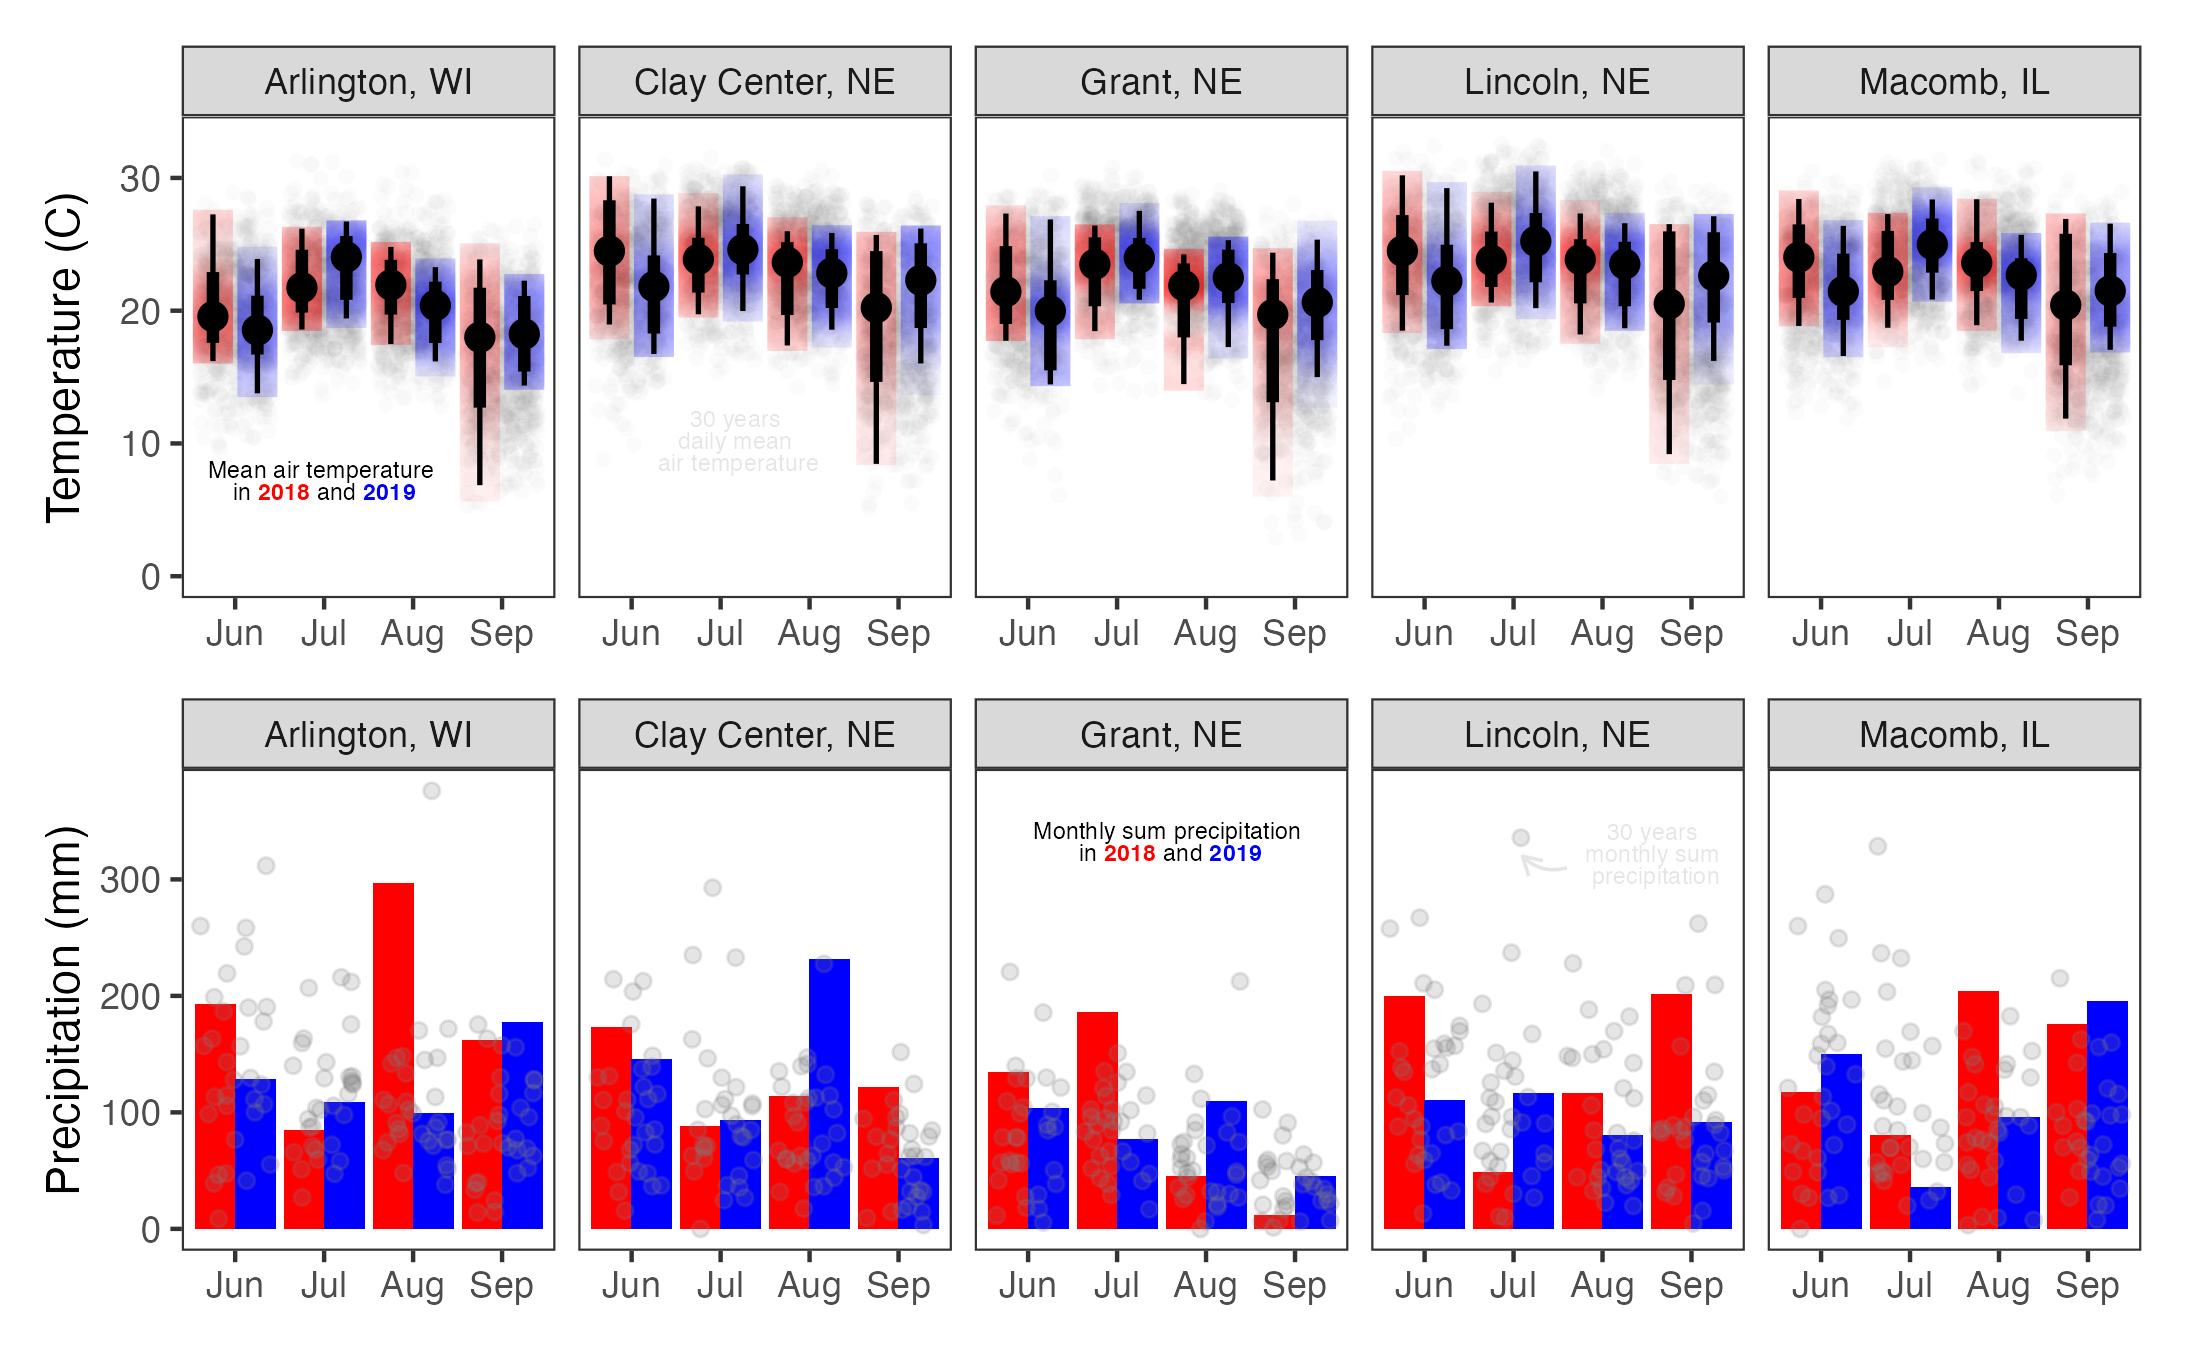
\includegraphics[width=160mm,height=100mm]{../data analysis/weather/Figure 1} 

}

\caption{Mean average temperature (C) and total montly precipitation (mm) at Arlington, WI, Clay Center, NE, Grant, NE, Lincoln, NE and Macomb, IL}\label{fig:Figure-1}
\end{figure}

\begin{figure}

{\centering 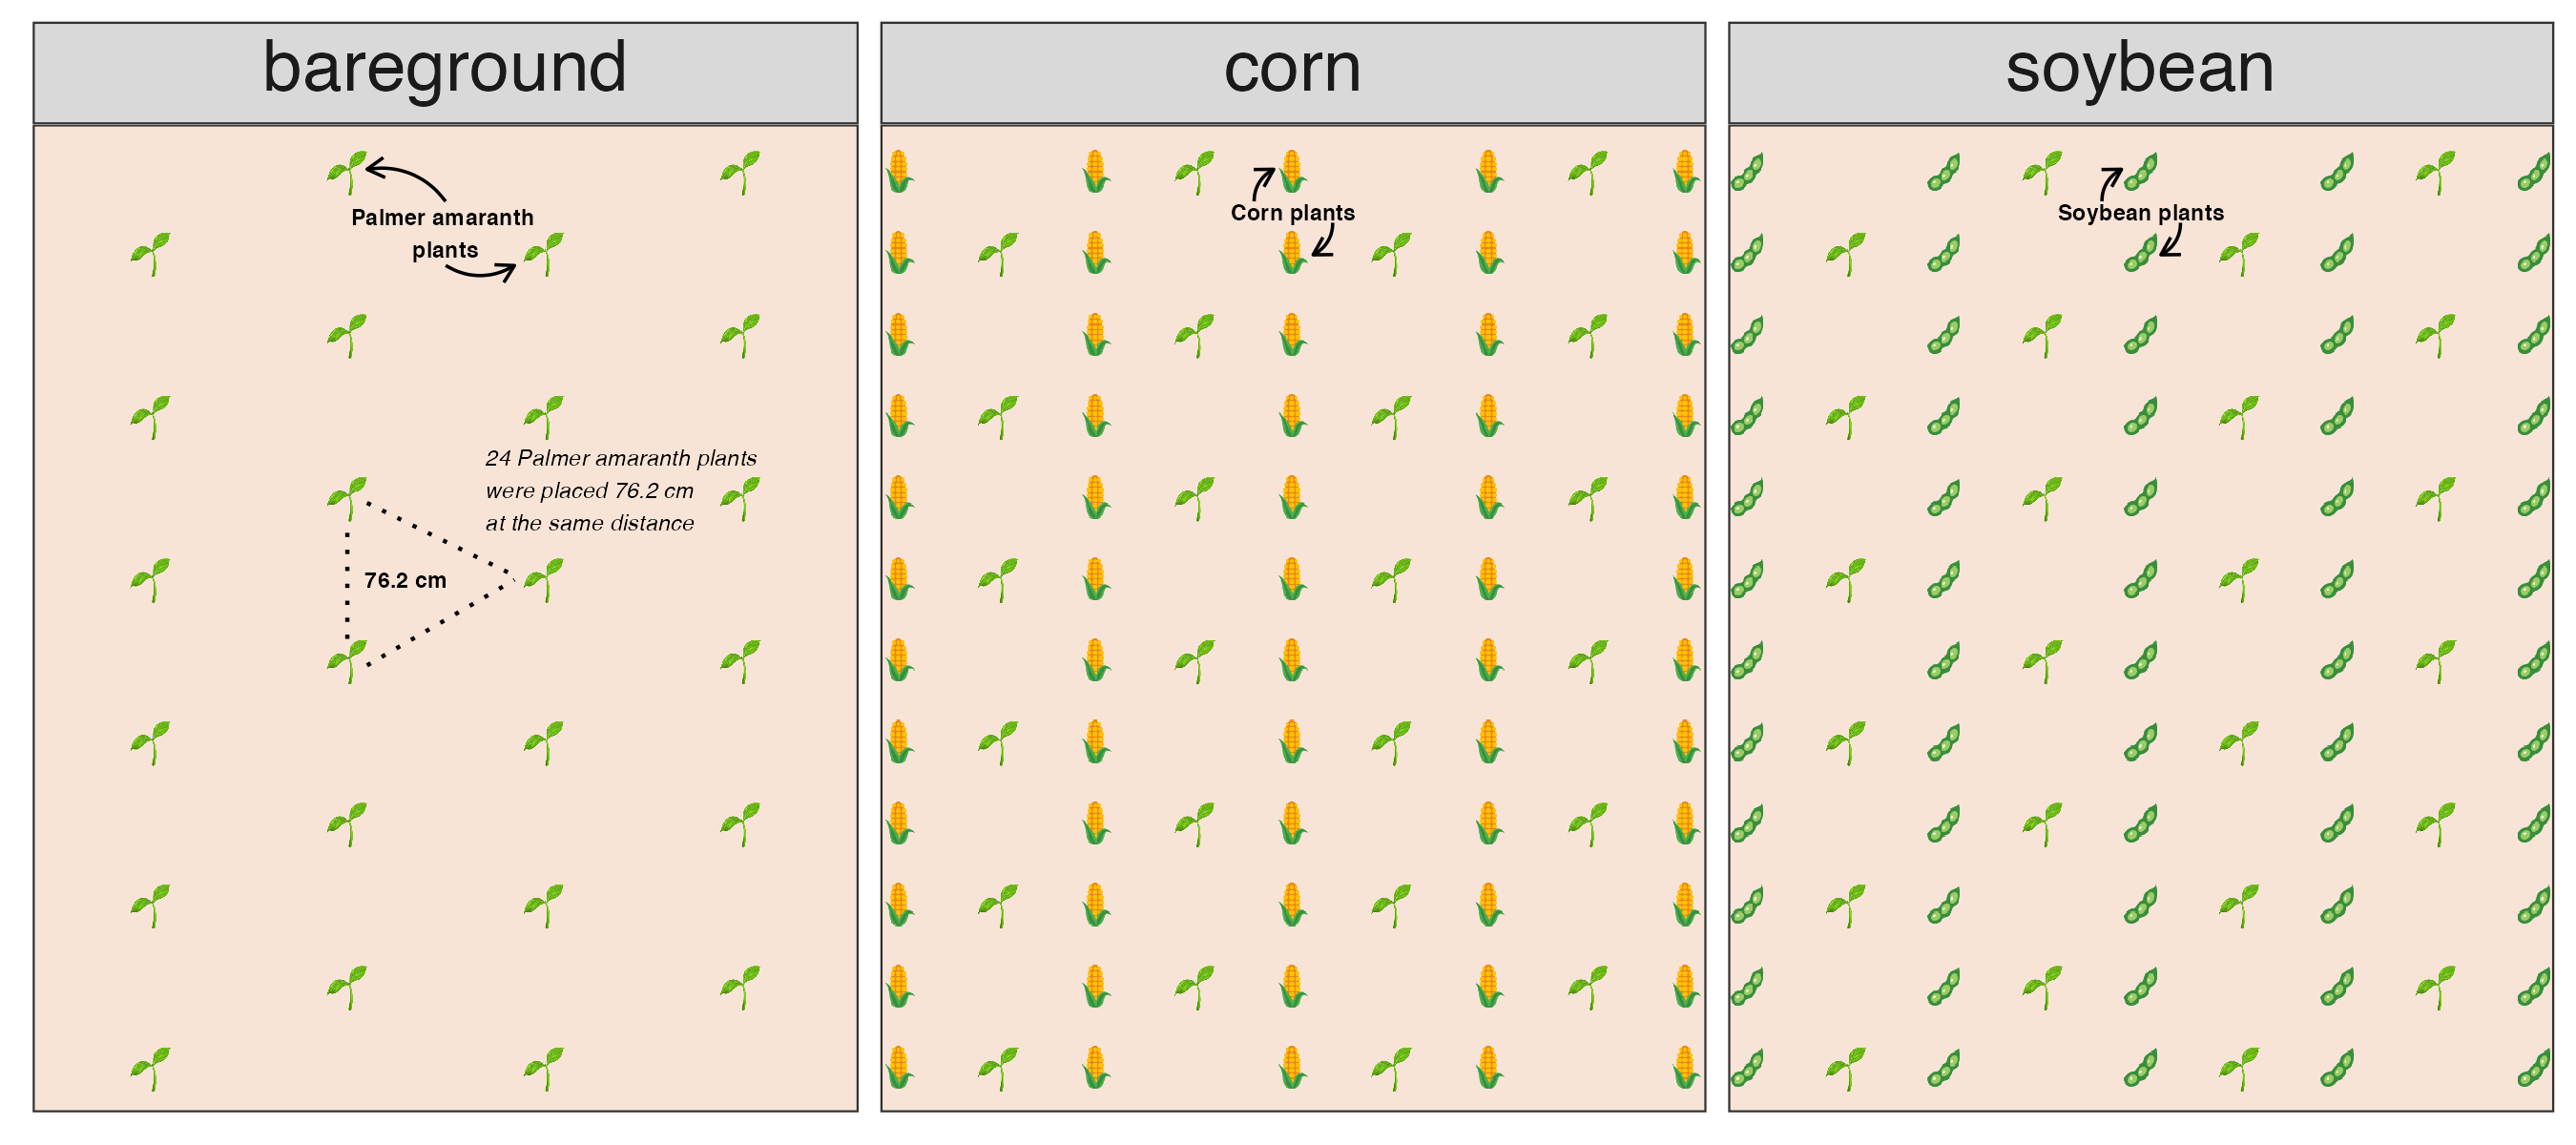
\includegraphics[width=150mm,height=70mm]{../data analysis/figures/Figure 2} 

}

\caption{Palmer amaranth adaptation study layout of a plant cohort timing in bareground, corn, and soybean. Twenty-four Palmer amaranth plants were place 76.2 cm apart in each field experimental unit}\label{fig:Figure-2}
\end{figure}

\begin{figure}

{\centering 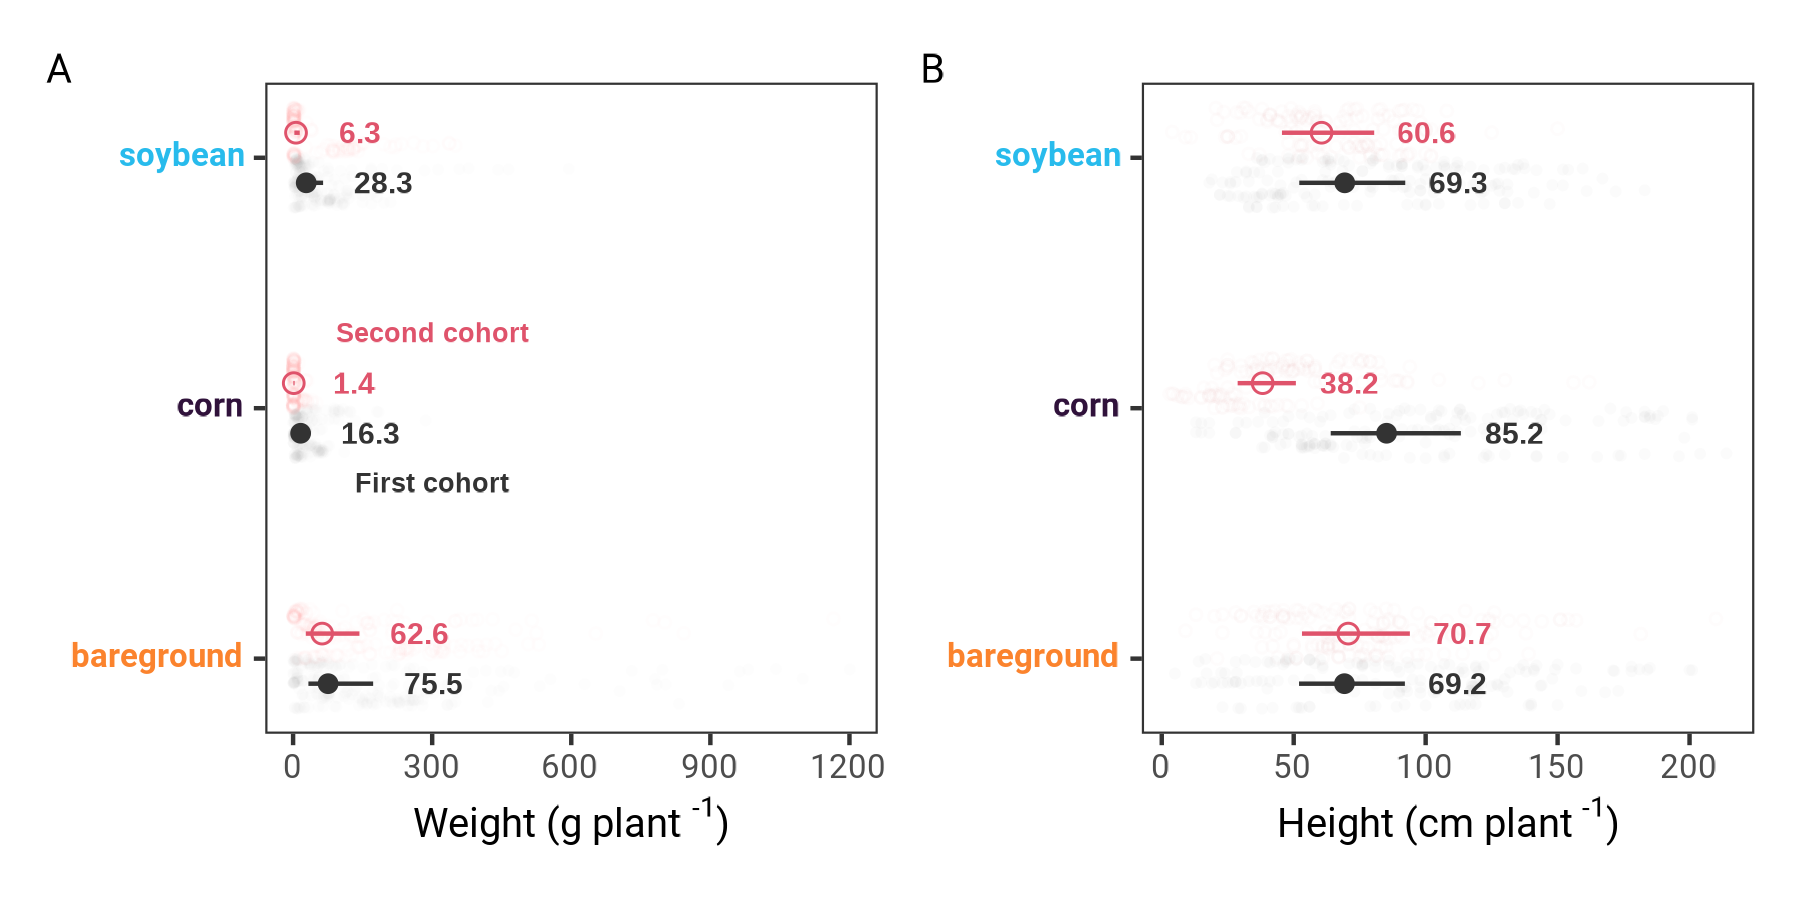
\includegraphics[width=150mm,height=90mm]{../data analysis/figures/Figure 3} 

}

\caption{Palmer amaranth biomass (A) and height (B) growing in corn, bareground, and soybean nested across Arlington, WI, Clay Center, NE, Grant, NE, Lincoln, NE and Macomb, IL}\label{fig:Figure-3}
\end{figure}

\begin{figure}

{\centering 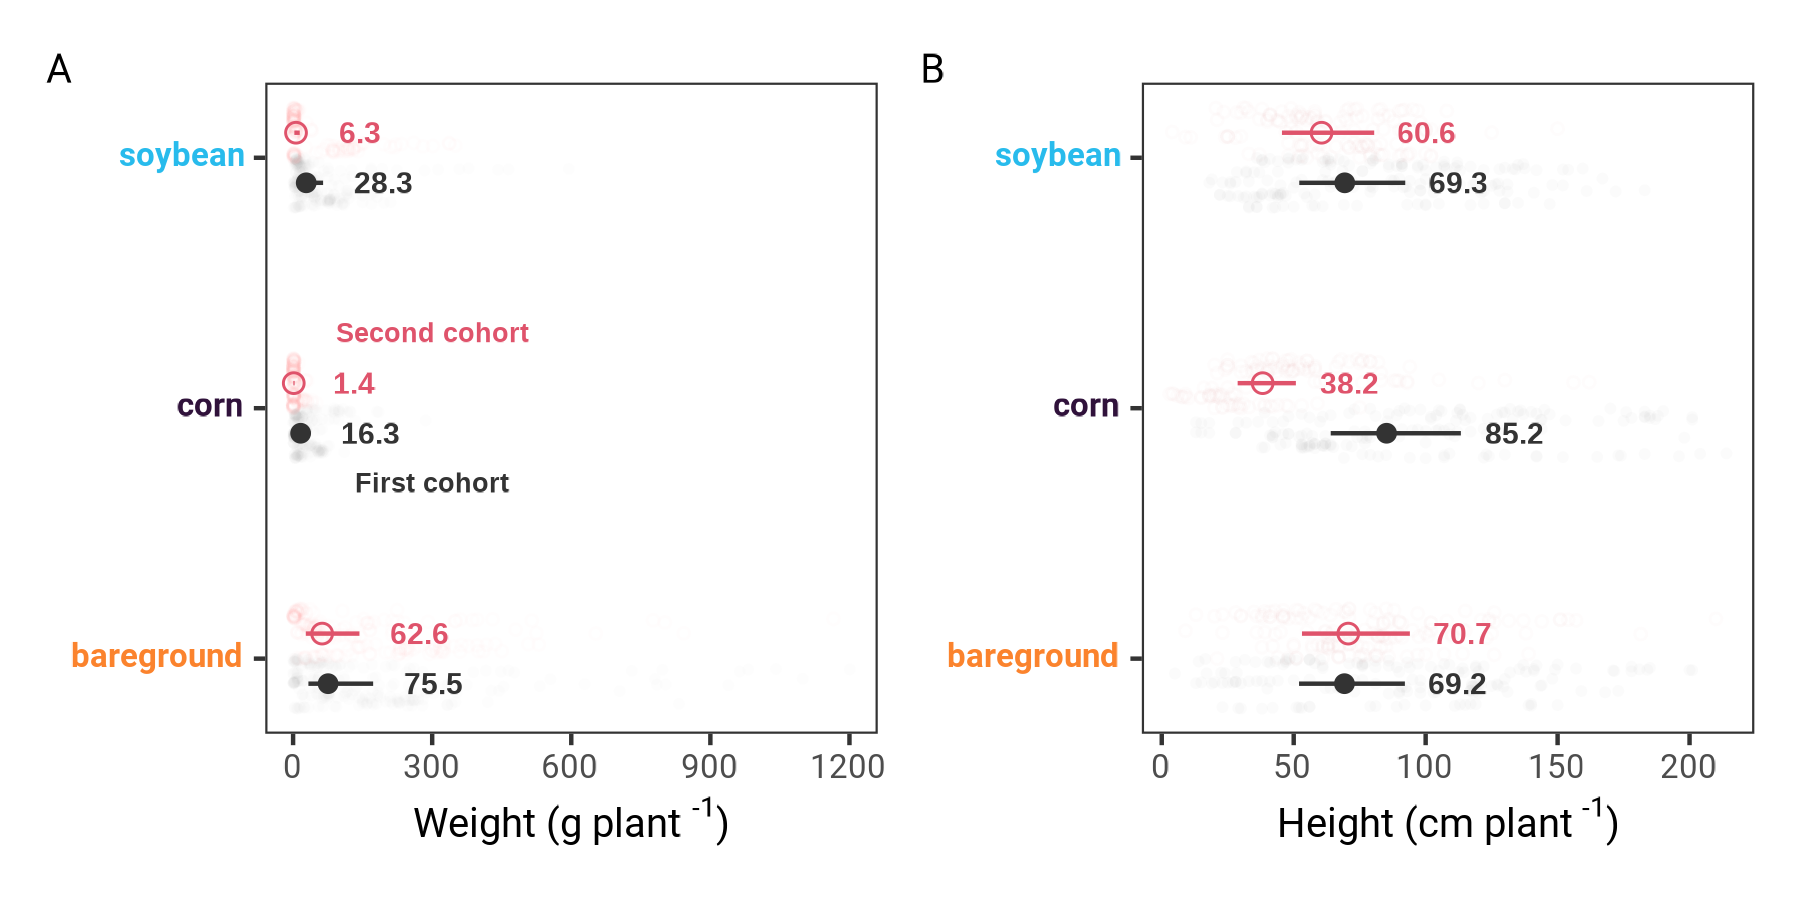
\includegraphics[width=150mm,height=150mm]{../data analysis/figures/Figure 4} 

}

\caption{Cumulative flowering of Palmer amaranth at first and second transplant timing (A) and day of year of 10, 50, and 90 cumulative flowering at first and second cohort transplanting time (B) nested across Arlington, WI, Clay Center, NE, Grant, NE, Lincoln, NE and Macomb, IL}\label{fig:Figure-4}
\end{figure}

\begin{figure}

{\centering 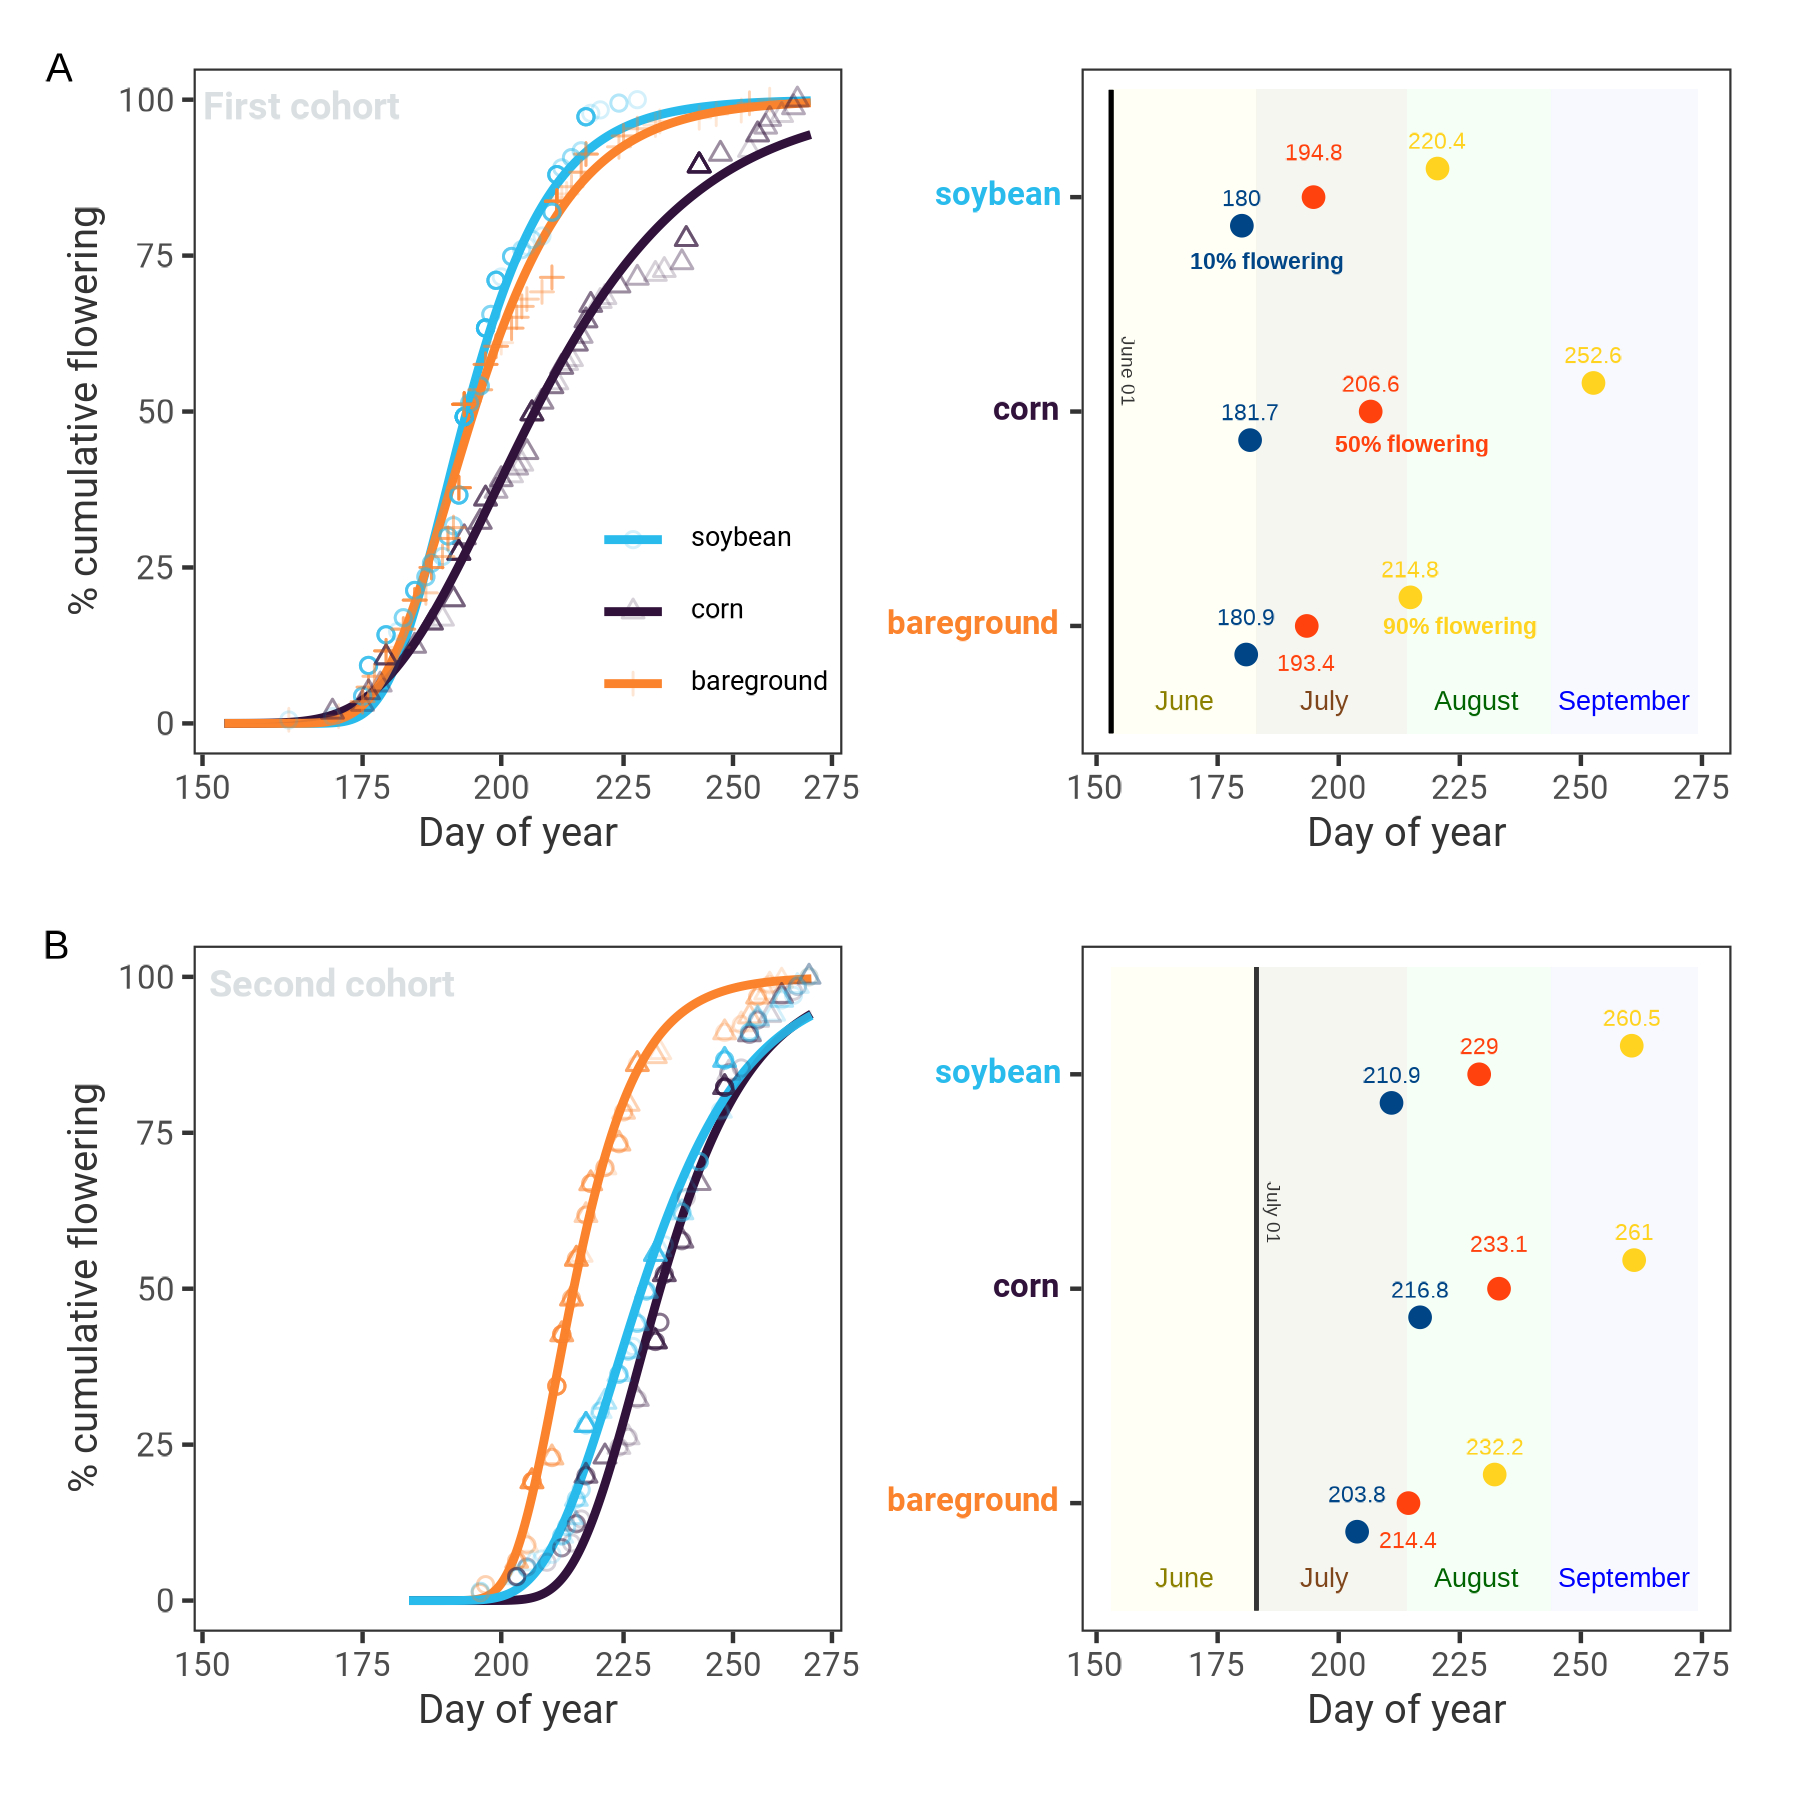
\includegraphics[width=170mm,height=70mm]{../data analysis/figures/Figure 5} 

}

\caption{The probability (P) of being female Palmer amaranth by day of year (A), weight (B), and height (C). Black line represents the model estimation and shaded green the confidence intervals}\label{fig:Figure-5}
\end{figure}

\begin{figure}

{\centering 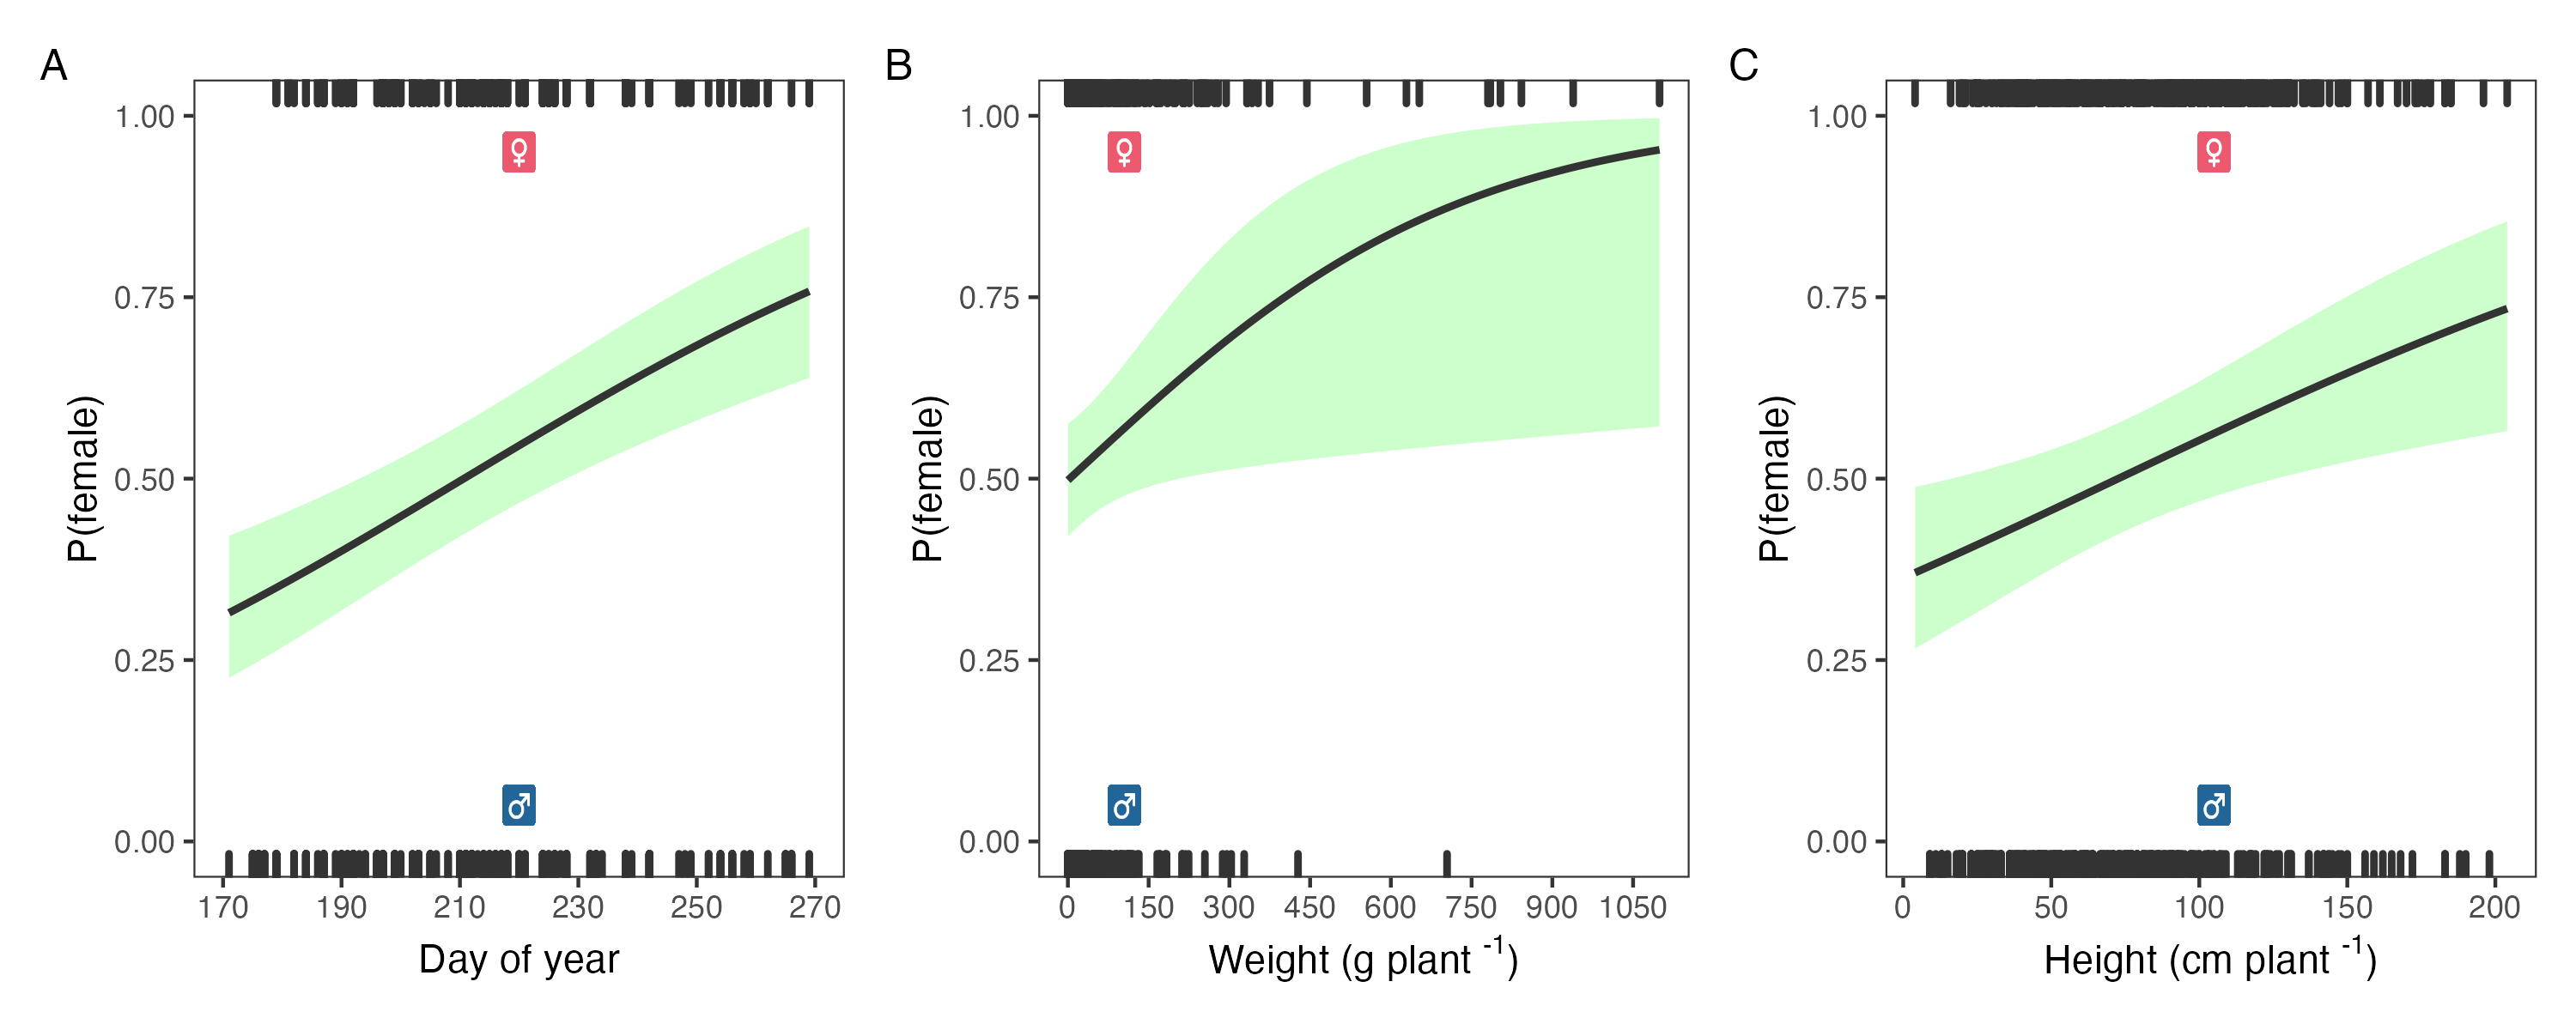
\includegraphics[width=150mm,height=90mm]{../data analysis/figures/Figure 6} 

}

\caption{MCO (180 cm) holds harvested Palmer amaranth plants at 40 days after first cohort transplanting (A) and 33 days after second cohort transplanting (B) time. From left to right in each image, Palmer amaranth growing in bareground, soybean and corn in Arlington, Wisconsin}\label{fig:Figure-6}
\end{figure}

\end{document}
